\chapter{Incompressible Navier-Stokes Solver}
\label{IncNSsolver}

\section{Synopsis}
A useful tool implemented in Nektar++ is the incompressible Navier
Stokes solver that allows one to solve the governing equation for
viscous Newtonians fluids governed by:

\begin{subequations}
\begin{align}
    \frac{\partial \mathbf{u}}{\partial t} + \mathbf{u} \cdot \nabla \mathbf{u} &= -\nabla p + \nu \nabla^2 \mathbf{u} +  \mathbf{f} \label{eqn.NSmom} \\
    \nabla \cdot \mathbf{u} &= 0
\end{align}
 \end{subequations}

where $\mathbf{u}$ is the velocity, $p$ is the specific pressure (including
density) and $\nu$ the kinematic viscosity.

Various approaches to solve and analyse this set of equations are 
available in Nektar\texttt{++} as shwon in table~\ref{tab.IncNSSolvers}.

\begin{table}
    \centering
\caption{An overview of the solvers available in Nektar++ for the incompressible Navier-Stokes equations.}
\begin{tabular}{ll}
    Solver & Options\\
    \toprule
    Velocity Correction Scheme & Semi-Implicit\\
    " & Semi-Implicit w/ Weak Pressure\\
    " & Implicit\\
    " & Coordinate Transformation \\
    Smoothed Profile Method & -\\
    Linear Stability Analysis & Direct \\
    " & Adjoint \\
    " & Transient Growth \\
    Steady-State solver & Selective Frequency Damping \\
    Direct (Coupled) Solver & Stokes Problem \\
\end{tabular}
\label{tab.IncNSSolvers}
\end{table}


\subsection{Velocity Correction Scheme}
\label{VCSScheme}
The first approach uses a splitting/projection method where the
velocity system and the pressure are typically
decoupled. Splitting schemes are typically favoured for their
numerical efficiency since the velocity and pressure are handled
independently, requiring the solution of four (in three dimensions)
elliptic systems of rank $N$ (opposed to a single system of rank $4N$
solved in the Stokes problem). However, a drawback of this approach is
the splitting scheme error which is introduced when decoupling the
pressure and the velocity system, although this can be made consistent
with the overall temporal accuracy of the scheme by appropriate
discretisation of the pressure boundary conditions.

The scheme discretises the momentum equation Eq.~\eqref{eqn.NSmom} with a backwards
approximation of the time derivative to obtain
\begin{equation}
  \frac{\partial \mathbf{u}}{\partial t}^{n+1} \simeq \frac{\gamma_0 \tilde{\mathbf{u}}^{n+1} - \hat{\mathbf{u}}}{\Delta t}
\end{equation}
where $\tilde{\mathbf{u}}^{n+1}$ is an intermediate velocity and $\hat{\mathbf{u}}$ 
is the summation of previous solutions.

With the discrete time derivative, we initially have to 
solve a pressure Poisson equation of the form
\begin{equation}
  \nabla^2 p^{n+1}=\nabla\cdot \Bigl(
  \frac{\hat{\mathbf{u}}}{\Delta t}  - \mathbf{N}^{*,n+1} \Bigr)
  \label{eqn.pressurepoisson}
\end{equation}
and use consistent Neumann boundary conditions prescribed as
\begin{equation}
  \frac{\partial p}{\partial n}^{n+1}= - \Bigl[ \frac{\partial \mathbf{u}}{\partial t}^{n+1} + \nu (\nabla \times \nabla \times   \mathbf{u})^{*,n+1} + \mathbf{N}^{*,n+1}\Bigr]\cdot \mathbf{n}
  \label{eqn.pressurebcs}
\end{equation}
Here, the advection term is denoted as 
$\mathbf{N}^{*,n+1} = [\mathbf{u} \cdot \nabla \mathbf{u}]^{\star,n+1}$ 
where the superscript indicates extrapolation from previous solutions.

The second step solves a Helmholtz problem for each 
new velocity component $[u^{n+1}, v^{n+1}, w^{n+1}]$
which leads us to
\begin{equation}
  \Bigl(\Delta-\frac{\gamma_0}{\nu \Delta t}\Bigr)\mathbf{u}^{n+1}=-\Bigl(\frac{\gamma_0}{\nu \Delta t}\Bigr)\hat{\mathbf{u}} + \frac{1}{\nu} \nabla p^{n+1}.
  \label{eqn.velocityhelm}
\end{equation}
This form of the Velocity Correction scheme is generally referred to as 
Semi-Implicit scheme, because diffusion terms are treated 
implicit while advection is treated explicit.

The algorithm follows the general structure outlined in figure~\ref{fig.VCSAlgorithm}.
Essentially, it solves for the new pressure $p^{n+1}$ and velocity $u^{n+1}$ 
based on initial conditions at $t^n = n \Delta t$ and boundary conditions. 
The three-step structure begins with evaluating the \textcolor{blue}{(explicit) advection terms}.
Next, a Poisson problem for the new \textcolor{red}{pressure $p^{n+1}$} is solved.
Finally, a Helmholtz problem is solved for each 
\textcolor{darkgreen}{velocity component} ($\textcolor{darkgreen}{\mathbf{u}^{n+1}=[u,v,w]^T}$ in 3D).

\begin{figure}[!htbp]
\centering
\begin{tikzpicture}
    \node[draw,align=center,color=blue] (Adv) [text width=2cm] at (0,0) {Advection $\mathbf{N}^{*,n+1}$};
    \node[draw,align=center,color=red] (P) [text width=2cm] at (0,-2) {Poisson $\nabla^2 p^{n+1}$};
    \node[draw,align=center,color=darkgreen] (H) [text width=3.5cm] at (0,-4) {3x Helmholtz $\lambda \mathbf{u}^{n+1} + \nabla^2 \mathbf{u}^{n+1}$};
    \node[rotate=90] (Tl) at (2.5,-2) {\small Time loop $n=n+1$};

    % Arrows
    \draw[-latex] (Adv) edge (P) (P) edge (H) (H) -- (2.7,-4) -- (2.7,0) -- (Adv);
\end{tikzpicture}
\label{fig.VCSAlgorithm}
\caption{The algorithm of the Velocity Correction scheme to 
compute pressure and velocity at the new time $t^n = n \Delta t$.}
\end{figure}


\subsubsection{Velocity Correction Scheme with a Weak Pressure formulation}
\label{VCSWeakScheme}

One way to improve the Velocity Correction scheme is the weak pressure formulation.
This form uses the same algorithm from figure~\ref{fig.VCSAlgorithm}.
However, the scheme uses the extrapolated advection term in the pressure forcing instead
of the boundary conditions.
This changes the pressure Poisson boundary condition 
from equation Eq.~\eqref{eqn.pressurebcs} to become
\begin{equation}
  \frac{\partial p}{\partial n}^{n+1}= - \Bigl[ \frac{\partial \mathbf{u}}{\partial t}^{n+1} + \nu (\nabla \times \nabla \times \mathbf{u})^{*,n+1}\Bigr]\cdot \mathbf{n}.
  \label{eqn.pressurebcsWeak}
\end{equation}
Further details for this scheme can be found in the Developer-Guide.

\subsubsection{Implicit Velocity Correction Scheme}
\label{VCSImplicitScheme}

% Introduction to the implicit scheme
The implicit solver handles the advection terms implicitly. 
Effectively, it uses the same formulation
as the Velocity Correction scheme described above, but brings the advection
operator on the left-hand side through a linearisation. 
The approach is similar to the work of \cite{Simo1994,Dong2010}.

The new velocity equation with linearised advection term is
\begin{equation}
    \Bigl(\Delta-\frac{\gamma_0}{\nu \Delta t} + \frac{1}{\nu} \tilde{\mathbf{u} \cdot \nabla}\Bigr)\mathbf{u}^{n+1}=-\Bigl(\frac{\gamma_0}{\nu \Delta t}\Bigr)\hat{\mathbf{u}} + \frac{1}{\nu} \nabla p^{n+1}
  \label{eqn.velocityadr}
\end{equation}

% Outline of the algorithm
The algorithm follows a similar structure to the Semi-Implicit 
algorithm introduced above in section~\ref{VCSScheme}.
The Poisson problem for the new \textcolor{red}{pressure $p^{n+1}$} is 
identical to the weak pressure formulation in section~\ref{VCSWeakScheme}.
The difference here is using an implicit advection operator that relaxes 
the Courant-Friedrichs-Levy (CFL) limitation for the time step size.
This results in an \textcolor{darkgreen}{Advection-Diffusion-Reaction (ADR)} problem for the new velocity components.

\begin{figure}[!htbp]
\centering
\begin{tikzpicture}
    \node[draw,align=center,color=blue] (Adv) [text width=2cm] at (0,0) {Advection $\mathbf{N}^{*,n+1}$};
    \node[draw,align=center,color=red] (P) [text width=2cm] at (0,-2) {Poisson $\nabla^2 p^{n+1}$};
    \node[draw,align=center,color=darkgreen] (H) [text width=4.5cm] at (0,-4) {3x ADR\\ $\lambda \mathbf{u}^{n+1} + \nabla^2 \mathbf{u}^{n+1} + \tilde{\mathbf{u}} \cdot \nabla \mathbf{u}^{n+1}$};
    \node[rotate=90] (Tl) at (2.7,-2) {\small Time loop $n=n+1$};

    % Arrows
    \draw[-latex] (Adv) edge (P) (P) edge (H) (H) -- (2.9,-4) -- (2.9,0) -- (Adv);
\end{tikzpicture}
\label{fig.VCSImplicitAlgorithm}
\caption{The algorithm of the Implicit Velocity Correction scheme using an 
ADR solve for the new velocity components $\mathbf{u}^{n+1}$.}
\end{figure}

% Few more details for possible solver options
The linearisation of the advection operator uses the 
approximation $[\mathbf{u} \cdot \nabla \mathbf{u}]^{n+1} \approx 
[\tilde{\mathbf{u}} \cdot \nabla \mathbf{u}]^{n+1}$ where $\tilde{\mathbf{u}}$
is an approximate advection velocity.
The advection velocity $\tilde{\mathbf{u}}$ is implemented in two forms.
The first form is referred to as \texttt{Extrapolated} as it is 
based on a simple extrapolation of previous velocity solutions \cite{Simo1994}.
The second form is called \texttt{Updated} and it is based on a 
pressure-equation residual that uses the updated pressure gradient $\nabla p^{n+1}$ \cite{Dong2010}.
They are defined respectively as,
\begin{align}
    \texttt{Extrapolated}\qquad\tilde{\mathbf{u}}^{n+1} &=
    \sum_q \frac{\alpha_q}{\gamma} \mathbf{u}^{n-q},\\
    \texttt{Updated}\qquad\tilde{\mathbf{u}}^{n+1} &=
    \sum_q \frac{\alpha_q}{\gamma} \mathbf{u}^{n-q} 
    - \frac{\Delta t}{\gamma} \left(
    \nabla p^{n+1}
    + [\mathbf{u} \cdot \nabla \mathbf{u}]^{n} 
    + \nu \nabla \times \mathbf{\omega}^{n}
    - \mathbf{f}^{n+1} \right).
\end{align}
The scheme defaults to \texttt{Extrapolated}, see 
the examples in section~\ref{s:incns:examples} for 
how to choose \texttt{Updated} instead.

% Few performance hints
Note that the advection matrix needs to be
updated for every time-step, this potentially leads to increased
computational cost when compared to the Semi-Implicit scheme.
Also, consider that the solver is linearly-implicit instead of fully-implicit.
This means that there are no sub iterations for each time step and 
thus no free parameters (e.g. tolerance) that need to be defined additionally.


\subsubsection{Coordinate Transformation}
\label{VCSCoordinateTransformation}
For some problems the physical coordinate system is not the most computationally-efficient.
In these cases, there is a coordinate transformation option for the Velocity Correction scheme that allows
mapping from the physical coordinates to a numerical coordinate system.
More details for this method can be found in the Developer Guide as well as examples on how to use it in section~\ref{s:incns:examples}.

\subsubsection{Substepping/subcycling the Velocity Correction Scheme}

It is possible to use different time steps in the velocity correction
scheme using a substepping (also known as subcycling) \cite{Sh03} or
auxiliary semi-Lagrangian approach \cite{XiShDoKa}. Originally the
scheme was proposed by Maday, Patera and Ronquist who referred to as
an operator-integration-factor splitting method \cite{MaPaRo}

\begin{figure}[!htbp]
\label{fig.substep}
  \centering
 {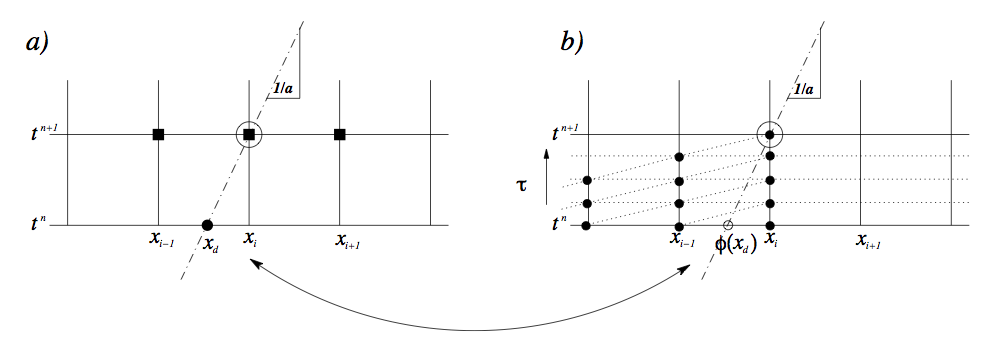
\includegraphics[width=1 \textwidth]{img/substepimage.png}}
   \caption {Schematic representation of the substepping approach. (a)
     Making an explicit time step the hyperbolic solution, travelling
     with a speed $a$, can be understood as being related to the
     solution at point $x_d$ (the departure point). (b) Making smaller
     explicit time steps we can evaluate the solution $\phi(x_d)$ at
     the departure point and then use this value to make a
     semi-Lagrangian discretisation of the implicit components usually
     associated with diffusion.}
\end{figure}


A schematic of the approach can be understood from figure~\ref{fig.substep}
where we observe that smaller time steps can be used
for the explicit advection steps whilst a larger overall time step is
adopted for the more expensive implicit solve for the diffusion
operator. More details of the implementation can be found in
\cite{XiShDoKa} and \cite{Sh03}. In the following sections we outline
the parameters that can be used to set up this scheme. Since the
explicit part is advanced using a DG scheme it is necessary to use a
\inltt{Mixed\_CG\_Discontinuous} expansion with this option.

\begin{notebox}
Some examples of the substepping scheme can be found in the regression tests
directory under
\texttt{\${NEKHOME}/Solver/IncNavierStokesSolver/Tests/} directory:
\texttt{KovaFlow\_SubStep\_2order.xml},
\texttt{Hex\_Kovasnay\_SubStep.xml} and
\texttt{Tet\_Kovasnay\_SubStep.xml}.
\end{notebox}
\subsection{Immersed Boundary Methods: Smoothed Profile Method}
\label{SPM}

The usual way to solve any PDE requires the definition of a well defined domain
where the solution is to be determined. Thus, for complex geometries, the
meshing process may get cumbersome and, in any case, the solver will have to
the meshing process may get cumbersome, and likely struggle to avoid the
presence of highly deformed and skewed elements. In addition, when solving
cases with moving boundaries, the mesh has to be updated every time step to
follow the shape of the boundaries, leading to a very resource and
time-consuming simulation that limits the capabilities of the solver.

Immersed Boundary Methods may be very useful in these situations, where the
definition of the boundaries requires a very complex mesh to reach
convergence. The main idea behind them is the use of a forcing term in the
incompressible Navier-Stokes equations in such a way that the mesh does not
necessariliy follow the boundaries. The solution in the regions falling outside
the boundaries is simply that of the boundaries, forcing the flow to behave as
if there were a real object even if the mesh does not represent it. The method
presented here is an adaptation of the Smoothed Profile Method
\cite{NakayamaSPM} extended to a high-order semi-implicit splitting scheme
\cite{LuoSPM, WangSPM}. This method ensures that the no-slip, no-penetration
and incompressibility constraints are mathematically enforced. Starting from
the incompressible Navier-Stokes equations, the term $\mathbf{f_s}$ is added to
the right hand side:

\begin{subequations}
\begin{equation} \label{spm:eq:SPMeqmov}
    \frac{\partial\mathbf{u}}{\partial t} + \mathbf{u}\cdot\nabla\mathbf{u} =
        -\nabla p + \nu\nabla^2\mathbf{u} + \mathbf{f} + \mathbf{f_s}
\end{equation}
\begin{equation}
    \nabla\cdot\mathbf{u} = 0
\end{equation}
\end{subequations}

The definition of this term depends on the method but, for the Smoothed Profile
Method (SPM), it is related to a \emph{shape function} $\Phi(\mathbf{x}, t)$
valued 0 in the fluid domain and 1 outside. It is usually defined as:

\begin{equation} 
    \Phi(\mathbf{x},t) = -\frac{1}{2} \left[ \tanh\left(\frac{d(\mathbf{x},t)}
        {\xi}\right)-1 \right],
\label{spm:eq:mask}
\end{equation}

\begin{figure}[!htbp]
    \centering
    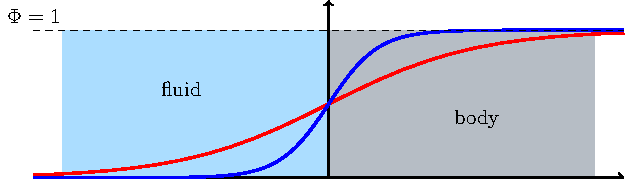
\includegraphics[width=0.7\textwidth]{img/concentration.pdf}
    \caption{Definition of the shape function $\Phi$ close to the boundary of
        an immersed body.}
    \label{spm:fig:shapefunc}
\end{figure}

being $\xi$ a scaling factor \cite{WangSPM} and $d(\mathbf{x}, t)$ a function
representing the distance to the boundary (positive inside the body, negative
inside the fluid). If the case to be simulated includes more than one immersed
boundaries, the final shape function is calculated by adding the individual
ones as long as they do not overlap:

\begin{equation}
    \Phi = \sum_i \Phi_i
\end{equation}

The approach followed during the implementation in \nekpp is an extension of
the Velocity Correction Scheme, using the final velocity obtained with this
method as an intermediate velocity to determine the value of the forcing term.
The initial equation Eq.~\eqref{spm:eq:SPMeqmov} is slightly modified and
integrated in time by means of a \emph{stiffly-stable} scheme and, then,
split into different smaller parts that are solved separately:

\begin{equation}
     \frac{\gamma_0\mathbf{u}^{n+1}-\sum_{q=0}^{J-1}\alpha_q~\mathbf{u}^{n-q}}
        {\Delta t} = -\sum_{q=0}^{J-1}\beta_q~(\mathbf{u}\cdot
        \nabla\mathbf{u})^{n-q} -\nabla (p^*+p_p)^{n+1} +
        \nu\nabla^2\mathbf{u}^{n+1} + \mathbf{f}^{n+1} + \mathbf{f_s}^{n+1}
\end{equation}

\begin{subequations}
\begin{gather}
    \frac{\mathbf{\tilde{u}}-\sum_{q=0}^{J-1}\alpha_q~\mathbf{u}^{n-q}}
        {\Delta t} = -\sum_{q=0}^{J-1}\beta_q~(\mathbf{u}\cdot
        \nabla\mathbf{u})^{n-q} + \mathbf{f}^{n+1},\\
    \frac{\mathbf{\hat{u}}-\mathbf{\tilde{u}}}{\Delta t} =
        -\nabla {p^*}^{n+1},\\[3mm]
    \frac{\gamma_0\mathbf{u^*}-\mathbf{\hat{u}}}{\Delta t} =
        \nu\nabla^2\mathbf{u}^{n+1},\\[3mm]
    \frac{\gamma_0\mathbf{u}^{n+1}-\gamma_0\mathbf{u^*}}{\Delta t} =
        -\nabla p_p^{n+1} + \mathbf{f_s}^{n+1}
\end{gather}
\end{subequations}

The new term $\mathbf{f_s}$ is defined as follows:

\begin{equation}
    \mathbf{f_s}^{n+1} = \frac{\gamma_0\Phi^{n+1}(\mathbf{u_p}^{n+1}-
        \mathbf{u^*})}{\Delta t},
\end{equation}

where $\alpha_q$, $\beta_q$ and $\gamma_0$ are coefficients of the
stiffly-stable time integration method and $\mathbf{u_p}$ is the velocity of
the points that lay outside the boundaries. Thus, the new term is just an
acceleration proportional to the difference between the expected and the
intermediate velocity, forcing the flow to follow the shapes defined by $\Phi$
and $\mathbf{u_p}$. 

\subsection{Linear Stability Analysis}

Hydrodynamic stability is an important part of fluid-mechanics that has a relevant role in understanding how an unstable flow can evolve into a turbulent state of motion with chaotic three-dimensional vorticity fields and a broad spectrum of small temporal and spatial scales. The essential problems of hydrodynamic stability were recognised and formulated in 19th century, notably by Helmholtz, Kelvin, Rayleigh and Reynolds.

Conventional linear stability assumes a normal representation of the perturbation fields that can be represented as independent wave packets, meaning that the system is self-adjoint. The main aim of the global stability analysis is to evaluate the amplitude of the eigenmodes as time grows and tends to infinity. However, in most industrial applications, it is also interesting to study the behaviour at intermediate states that might affects significantly the functionality and performance of a device. The study of the transient evolution of the perturbations is seen to be strictly related to the non-normality of the linearised Navier-Stokes equations, therefore the normality assumption of the system is no longer assumed. The eigenmodes of a non-normal system do not evolve independently and their interaction is responsible for a non-negligible transient growth of the energy. Conventional stability analysis generally does not capture this behaviour, therefore other techniques should be used.

A popular approach to study the hydrodynamic stability of flows consists in performing a direct numerical simulation of the linearised Navier-Stokes equations using iterative methods for computing the solution of the associated eigenproblem. However, since linearly stable flows could show a transient increment of energy, it is necessary to extend this analysis considering the combined effect of the direct and adjoint evolution operators. This phenomenon has noteworthy importance in several engineering applications and it is known as transient growth.

In Nektar++ it is then possible to use the following tools to perform stability analysis:

\begin{itemize}
\item direct stability analysis;
\item adjoint stability analysis;
\item  transient growth analysis;
\end{itemize}

\subsubsection{Direct stability analysis}


The equations that describe the evolution of an infinitesimal disturbance in the
flow can be derived decomposing the solution into a basic state $(\mathbf{U},
p)$ and a perturbed state  $\mathbf{U}+\varepsilon \mathbf{u'}$ with
$\varepsilon \ll 1$ that both satisfy the Navier-Stokes equations. Substituting
into the Navier-Stokes equations and considering that the quadratic terms $\mathbf{u'} \cdot \nabla \mathbf{u'}$ can be neglected, we obtain the linearised Navier-Stokes equations:

\begin{subequations}
\begin{equation}
  \frac{\partial \mathbf{u'}}{\partial t} + \mathbf{U} \cdot  \nabla \mathbf{u'}+\mathbf{u'} \cdot \nabla \mathbf{U} = -\nabla p + \nu \nabla^2 \mathbf{u'} + \mathbf{f}
\end{equation}

\begin{equation}
    \nabla \cdot \mathbf{u'} = 0
\end{equation}

\end{subequations}



The linearised Navier-Stokes equations are identical in form to the non-linear equation, except for the non-linear advection term. Therefore the numerical techniques used for solving Navier-Stokes equations can still be applied as long as the non-linear term is substituted with the linearised one. It is possible to define the linear operator that evolved the perturbation forward in time:

\begin{equation}
   \mathbf{u'}(\mathbf{x},t)=\mathcal{A}(\mathbf{U})\mathbf{u'}(\mathbf{x},0)
\end{equation}

Let us assume that the base flow  $\mathbf{U}$ is steady, then the perturbations are autonomous and we can assume that:

\begin{equation}
   \mathbf{u'}(\mathbf{x},t)=\mathbf{q'}(\mathbf{x})\exp(\lambda t) \quad \mbox{where} \, \lambda=\sigma+i \omega
\end{equation}

Then we obtain the associated eigenproblem:

\begin{equation}
   \mathcal{A}(\mathbf{U})\mathbf{q'}=\lambda \mathbf{q'}
\end{equation}

The dominant eigenvalue determines the behaviour of the flow. If the real part
is positive then there exist exponentially growing solutions. Conversely, if all
the eigenvalues have negative real part then the flow is linearly stable. If the real part of the eigenvalue is zero, it is a bifurcation point.

\subsubsection{Adjoint Stability Analysis}

The adjoint of a linear operator is one of the most important concepts in
functional analysis and it plays an important role in understanding transition to turbulence. Let us write the linearised Navier-Stokes equation in a compact form:

\begin{equation}
\mathcal{H}\mathbf{q}=0 \quad \mbox{where} \quad \mathcal{H}=\left( \begin{array}{c|c}
  -\partial_t-(\mathbf{U} \cdot \nabla)+ (\nabla \mathbf{U}) \cdot + \frac{1}{Re} \nabla^2 & -\nabla \\
  \hline
  \nabla \cdot  & 0
   \end{array}
 \right)
 \end{equation}


The adjoint operator $\mathcal{H}^*$ is defined as:

\begin{equation}
\left \langle \mathcal{H}\mathbf{q}, \mathbf{q} \right \rangle= \left \langle \mathbf{q}, \mathcal{H}^*\mathbf{q}^* \right \rangle
\end{equation}

Integrating by parts and employing the divergence theorem, it is possible to express the adjoint equations:

\begin{subequations}
\begin{equation}
-\frac{\partial \mathbf{u}^*}{\partial t}+(\mathbf{U} \cdot \nabla)\mathbf{u}^*+(\nabla \mathbf{U})^T \cdot \mathbf{u}^*=-\nabla p^*+\frac{1}{Re} \nabla^2 \mathbf{u}
\end{equation}

\begin{equation}
\nabla \cdot \mathbf{u}^*=0
\end{equation}
\end{subequations}

The adjoint fields are in fact related to the concept of \textbf{receptivity}. The value of the adjoint velocity at a point in the flow indicates the response that arises from an unsteady momentum source at that point. The adjoint pressure and the adjoint stream function play instead the same role for mass and vorticity sources respectively. Therefore, the adjoint modes can be seen as a powerful tool to understand where to act in order to ease/inhibit the transition.

\subsubsection{Transient Growth Analysis}

Transient growth  is a phenomenon that occurs when a flow that is linearly stable, but whose perturbations exhibit a non-negligible transient response due to regions of localised convective instabilities. This situation is common in many engineering applications, for example in open flows where the geometry is complex, producing a steep variation of the base flow. Therefore, the main question to answer is if it exists a bounded solution that exhibit large growth before inevitably decaying. Let us introduce a norm to quantify the size of a perturbation. It is physically meaningful to use the total kinetic energy of a perturbation on the domain $\Omega$. This is convenient because it is directly associated with the
standard-$L2$ inner product:

\begin{equation}
\mathcal{A}(\tau)\mathbf{v}=\sigma \mathbf{u}, \quad \left\| \mathbf{u} \right\|=1
\end{equation}


where $\sigma=\left\| \mathbf{u'}(\tau)\right\|$. This is no other
than the singular value decomposition of $\mathcal{A}(\tau)$. The
phenomenology of the transient growth can be explained considering the
non-normality of the linearised Navier-Stokes evolution operator. This
can be simply understood using the simple geometric example showed in
figure~\ref{TG}. Let us assume a unit-length vector $\mathbf{f}$
represented in a non-orthogonal basis .This vector is defined as the
difference of the nearly collinear vectors $\mathbf{\Phi_1}$ and
$\mathbf{\Phi_2}$.  With the time progression, the component of these
two vectors decrease respectively by 20\% and 50\%. The vector
$\mathbf{f}$ increases substantially in length before decaying to
zero. Thus, the superposition of decaying non-orthogonal eigenmode can
produce in short term a growth in the norm of the perturbations.


\begin{figure}[!htbp]
\centering
 \label{TG}
 {\includegraphics[width=1 \textwidth]{img/transient_growth.png}}
   \caption {Geometric interpretation of the transient growth. Adapted from Schmid, 2007 }
\end{figure}


\subsection{Steady-state solver using Selective Frequency Damping}
\label{SectionSFD}

To compute linear stability analysis, the choice of the base flow,
around which the system will be linearised, is crucial. If one wants
to use the steady-state solution of the Navier-Stokes equations as
base flow, a steady-state solver is implemented in \nekpp. The method
used is the encapsulated formulation of the Selective Frequency
Damping method \cite{JoCoSh14}. Unstable steady base flows can be
obtained with this method. The SFD method is based on the filtering
and control of unstable temporal frequencies within the flow. The time
continuous formulation of the SFD method is
\begin{equation}
\begin{cases}
\dot{q}=NS(q)-\chi (q-\bar{q}), \\
\dot{\bar{q}}=\frac{q-\bar{q}}{\Delta}.
\end{cases}
\label{SFD-General}
\end{equation}
where $q$ represents the problem unknown(s), the dot represents the time derivative, $NS$ represents the Navier-Stokes equations, $\chi \in \mathbb{R}_+$ is the control coefficient, $\bar{q}$ is a filtered version of $q$, and $\Delta \in \mathbb{R}_+ ^*$ is the filter width of a first-order low-pass time filter. The steady-state solution is reached when $q=\bar{q}$.

The convergence of the method towards a steady-state solution depends on the choice of the parameters $\chi$ and $\Delta$. They have to be carefully chosen: if they are too small, the instabilities within the flow can not be damped; but if they are too large, the method may converge extremely slowly. If the dominant eigenvalue of the flow studied is known (and given as input), the algorithm implemented can automatically select parameters that ensure a fast convergence of the SFD method. Most of the time, the dominant eigenvalue is not know, that is why an adaptive algorithm that adapts $\chi$ and $\Delta$ all along the solver execution is also implemented.

Note that this method can not be applied for flows with a pure exponential growth of the instabilities (\textit{e.g.} jet flow within a pipe). In other words, if the frequency of the dominant eigenvalue is zero, then the SFD method is not a suitable tool to obtain a steady-state solution.


\subsection{Direct solver (coupled approach)}
\label{DirectSolv}
The second approach consists of directly solving the matrix problem
arising from the discretization of the Stokes problem.  The direct
solution of the Stokes system introduces the problem of appropriate
spaces for the velocity and the pressure systems to satisfy the
inf-sup condition and it requires the solution of the full
velocity-pressure system. However, if a discontinuous pressure space
is used then all but the constant mode of the pressure system can be
decoupled from the velocity. When implementing this
approach with a spectral/hp element discretization, the remaining
velocity system may then also be statically condensed to decouple the so
called interior elemental degrees of freedom, reducing the Stokes
problem to a smaller system expressed on the elemental boundaries. The
direct solution of the Stokes problem provides a very natural setting
for the solution of the pressure system which is not easily dealt with
in a splitting scheme. Further, the solution of the full coupled
velocity system allows the introduction of a spatially varying
viscosity, which arise for non-Newtonian flows, with only minor
modifications.

\begin{notebox}
  The coupled solver is only supported for two-dimensional or quasi-3D problems,
  and only using a direct solver (e.g. \inltt{DirectStaticCond}) which prevents
  its use in parallel.
\end{notebox}

We consider the weak form of the Stokes problem for the velocity field
$\boldsymbol{u}=[u,v]^{T}$ and the pressure field $p$:

\begin{subequations}
\begin{equation}
 (\nabla \phi,\nu \nabla \boldsymbol{u}) - (\nabla\cdot\phi,p)=(\phi,\boldsymbol{f})
\end{equation}
\begin{equation}
 (q,\nabla \cdot \boldsymbol{u}) = 0
\end{equation}
\end{subequations}

where the components of $A$,$B$ and $C$ are
$\nabla\phi_b,\nu\nabla\boldsymbol{u_b}$,
$\nabla\phi_b,\nu\nabla\boldsymbol{u_i}$ and
$\nabla\phi_i,\nu\nabla\boldsymbol{u_i}$ and the components $D_b$ and
$D_i$ are $q,\nabla\boldsymbol{u_b}$ and $q,\nabla\boldsymbol{u_i}$.
The indices $b$ and $i$ refer to the degrees of freedom on the
elemental boundary and interior respectively. In constructing the
system we have lumped the contributions form each component of the
velocity field into matrices $A$,$B$ and $C$. However, we note that
for a Newtonian fluid the contribution from each field is
decoupled. Since the interior degrees of freedom of the velocity field
do not overlap, the matrix $C$ is block diagonal and to take advantage
of this structure we can statically condense out the $C$ matrix to
obtain the system:

\begin{equation}
\left[ \begin{array}{ccc}
 A-BC^{-1}B^T & D_b^T-BC^{-1}D_i & 0\\
 D_b-D_i^TC^{-1}B^T & -D_i^TC^{-1}D_i & 0\\
 B^T & D_i & C
 \end{array}\right]
 \left[ \begin{array}{c}
 \boldsymbol{u_b}\\
 p\\
 \boldsymbol{u_i}
 \end{array}\right] =
 \left[ \begin{array}{c}
 \boldsymbol{f_b} - BC^{-1}\boldsymbol{f_i}\\
 -D_i^TC^{-1}\boldsymbol{f_i}\\
 \boldsymbol{f_i}
 \end{array}\right]
 \end{equation}

 To extend the above Stokes solver to an unsteady Navier-Stokes solver
 we first introduce the unsteady term, $\partial
 \boldsymbol{u}/\partial t$, into the Stokes problem.  This has the
 principal effect of modifying the weak Laplacian operator
 $\nabla\phi,\nu\nabla\boldsymbol{u}$] into a weak Helmholtz operator
   $\nabla\phi,\nu\nabla\boldsymbol{u})-\lambda(\phi,\boldsymbol{u}$
   where $\lambda$ depends on the time integration scheme. The second
   modification requires the explicit discretisation of the non-linear
   terms in a similar manner to the splitting scheme and this term is
   then introduced as the forcing term $\boldsymbol{f}$. For more details see \cite{AiSh,ShAi}.



\section{Usage}

To run the incompressible solver in serial:
\begin{lstlisting}[style=BashInputStyle]
IncNavierStokesSolver mesh.xml session.xml -v 
\end{lstlisting}
%
where \inltt{IncNavierStokesSolver} is the name of the executable, \inltt{mesh.xml} is the name of the file that inlcudes all the high-order mesh information, \inltt{session.xml} is the name of the file that describes the polynomial expansions for the pressure and velocity fields, the boundary conditions and the numerical configuration of the problem. It is recommend to use the \inltt{-v}, or \inltt{--verbose} flag which activates additional information to be printed upon execution of the executable. It is possible to have the information from \inltt{mesh.xml} and \inltt{session.xml} in a single file, for example \inltt{meshAndSession.xml}. This compact format for the problem set-up is useful for small size problems and the previous command will look like:
\begin{lstlisting}[style=BashInputStyle]
IncNavierStokesSolver meshAndSession.xml -v 
\end{lstlisting}

In \emph{Nektar++}, it is possible to restart a simulation from an existing pressure and velocity field. In this scenario, the simulation will resume from the latest available time-step in the restart field and the numbering of the output checkpoint files will continue from the latest index. To avoid this and set the start time of the simulation and/or the index numbering of the checkpoint files one can use: 
\begin{lstlisting}[style=BashInputStyle]
IncNavierStokesSolver meshAndSession.xml -v --set-start-time 0 --set-start-chknumber 0
\end{lstlisting}
%
where the flag \inltt{--set-start-time} receives float values that set the starting time of the simulation and the flag \inltt{--set-start-chknumber} receives int values that specify the starting index for the output checkpoint files regardless of the settings introduced by the initialization field.
%
\begin{notebox}
If you want to run the IncNavierStokesSolver process in the background, so that you continue using the existing terminal, then you can use the following: \\ 
\texttt{IncNavierStokesSolver meshAndSession.xml -v > logAndErr.IncNS \&} \\
%
In this command, the \texttt{> logAndErr.IncNS} is specified to dump all the information that is printed from the executable inside the \inltt{logAndErr.IncNS} file and the error information in case an error shows up, the $\&$ symbol is responsible for launching the process in the background. This way, the current terminal can be used for different actions and the job will continue to run, even if the user loses connection from the terminal that the process was launched. To monitor the progress of the simulation and how far it is from completion when the process is running in the background: \\
\texttt{tail -f logAndErr.IncNS}
\end{notebox}

If \emph{Nektar++} is compiled with HDF5 support, then the output fields can be exported in compressed HDF5 format using the follwing command:
\begin{lstlisting}[style=BashInputStyle]
IncNavierStokesSolver mesh.xml session.xml -v -i Hdf5
\end{lstlisting}
%
where the flag \inltt{-i} or \inltt{--io-format Hdf5} enables the \inltt{IncNavierStokesSolver} executable to write the velocity and the pressure fields in HDF5. For large scale problems where the number of elements is above one million, it is recommended to convert the mesh in compressed HDF5 format and use the flag \inltt{--use-hdf5-node-comm} to enable loading the mesh in parallel and avoid running out of memory, in case of serial partitioning, as shown below:  
\begin{lstlisting}[style=BashInputStyle]
IncNavierStokesSolver mesh.xml session.xml -v -i Hdf5 --use-hdf5-node-comm
\end{lstlisting}
%
If \emph{Nektar++} is configured to run in parallel as described in Section~\ref{comp_test}, then the following command is used: 
\begin{lstlisting}[style=BashInputStyle]
 mpirun -np 10 IncNavierStokesSolver mesh.xml session.xml -v 
\end{lstlisting}

where \inltt{mpirun} can be replaced by \inltt{mpiexec} depending on the MPI protocol that is available in the system and $10$ is the number of the requested processors. A detailed summary of all the available flags is written in Section~\ref{command_line}. 
%
\begin{notebox}
To list all the available flags for the \texttt{IncNavierStokesSolver} executable, run: \\ 
\texttt{IncNavierStokesSolver -h} \\
\end{notebox}

\section{Setting up the Simulation}
\label{VCSSetup}

In the following the possible options are shown for setting up a simulation using
the incompressible Navier-Stokes.

\subsection{Expansions and Approximation Spaces}
The \texttt{Expansions} are introduced generally in section~\ref{sec:xml:expansions}.
The \texttt{Expansion} section for an incompressible flow
simulation can be set as for other solvers regardless of the projection type.
Here an example for a 3D simulation with all variables having a same polynomial 
order (for 2D simulations the specified fields
would be just \inltt{u,v,p}).

\begin{lstlisting}[style=XMLStyle]
<EXPANSIONS>
  <E COMPOSITE="C[0]" NUMMODES="6" FIELDS="u,v,w,p" TYPE="MODIFIED" />
</EXPANSIONS>
\end{lstlisting}

In case of a simulation using the Direct Solver we need to set
\inltt{FIELDS=u,v} as the pressure expansion order will be automatically set to
fulfil the inf-sup condition. Possible choices for the expansion \inltt{TYPE}
are:
\begin{center}
%\footnotesize
\small
\begin{tabular}{lcc}
\toprule
{Basis} & {\texttt{TYPE}} \\
\midrule
\texttt{Modal} & \texttt{MODIFIED} \\
\texttt{Nodal} & \texttt{GLL\_LAGRANGE} \\
\texttt{Nodal SEM} & \texttt{GLL\_LAGRANGE\_SEM} \\
\bottomrule
\end{tabular}
\end{center}

For well resolved simulations it appears that often using the same
polynomial space for the pressure and velocity does give suitable
answer but this does not satisfy the so-called LBB or inf-sup
condition. Therefore, it is potentially better to specify an equivalent
of the \textbf{Taylor Hood} approximation and use one higher polynomial order
for velocity than the pressure with a continuous expansion. To specify
this type of expansion you can use an expansion section of the form:

\begin{lstlisting}[style=XMLStyle]
  <EXPANSIONS>
        <E COMPOSITE="C[0]" NUMMODES="8" FIELDS="u,v" TYPE="MODIFIED" />
        <E COMPOSITE="C[0]" NUMMODES="7" FIELDS="p"   TYPE="MODIFIEDQUADPLUS1" />
  </EXPANSIONS>
\end{lstlisting}

In the above example the ``u,v'' fields are specified to have a
polynomial order of 7 using a modified expansion. Implicitly this form
of the expansion definition uses a quadrature order of 9. The above
definition then also uses a modified expansion for pressure but of polynomial
order 6. Since currently for this solver to run we need to use a
consistent quadrature order for both the velocity and pressure fields
we specify the \inltt{MODIFIEDQUADPLUS1} to tell the solver to use an
additional quadrature point and therefore also use 9 quadrature points in
each 1D direction for the pressure. 

In other cases it is sometimes useful to run with an even higher
quadrature order, for example to handle highly deformed elements where
the Jacobian is represented by a polynomial expansion. This can be done
by using a more detailed definition of the expansion of the form:


\begin{lstlisting}[style=XMLStyle]
  <EXPANSIONS>
      <E COMPOSITE="C[0]" BASISTYPE="Modified_A,Modified_B" NUMMODES="8,8" POINTSTYPE="GaussLobattoLegendre,GaussRadauMAlpha1Beta0" NUMPOINTS="9,8"  FIELDS="u,v" />
      <E COMPOSITE="C[0]" BASISTYPE="Modified_A,Modified_B" NUMMODES="7,7" POINTSTYPE="GaussLobattoLegendre,GaussRadauMAlpha1Beta0" NUMPOINTS="9,8"  FIELDS="p" />
  </EXPANSIONS>
\end{lstlisting}

In this example we have specified an 8th order expansion for ``u,v''
and a 7th order expansion for ``p''. The BasisType is given as
``Modified\_A, Modified\_B'' which is for a triangular expansion (note that for
a quadrilateral expansion it would have been ``Modified\_A,Modified\_A'')
and so the number of quadrature points in this case is 9 in the first
direction which uses Gauss-Lobatto-Legendre points but only 8 in the
second direction since this uses a Gauss-Radau formula with
$\alpha=1,\beta=0$ weights (see \cite{KaSh05} for details).

Further information is also available in Section~\ref{sec:xml:expansions}.

\subsection{Governing Equation}
\label{incns:governingEq}
The first thing in setting up a simulation is to define what governing eqautions
are to be solved. This can be done using the \inltt{EqType} tag in the
\inltt{SOLVERINFO} section.      

Possible values are:
\begin{center}
\footnotesize
\renewcommand\arraystretch{1.2}
\begin{tabular}{lccccc}
\toprule
{Equations} & {\texttt{EQTYPE}} &{Dim.}&{Projections} & Alg.\\
\midrule
Steady Stokes (SS)& \texttt{SteadyStokes} & All & CG &VCS \\
Steady Oseen (SO) & \texttt{SteadyOseen} & All & CG& DS \\
Unsteady Stokes (US) & \texttt{UnsteadyStokes} & All & CG &VCS \\
Steady Linearised NS (SLNS) & \texttt{SteadyLinearisedNS} & All & CG & DS \\
Unsteady Linearised NS (ULNS) & \texttt{UnsteadyLinearisedNS} & All & CG & VCS,DS \\
Unsteady NS (UNS) & \texttt{UnsteadyNavierStokes} & All & CG,CG-DG & VCS\\
\bottomrule
\end{tabular}
\end{center}

For example, for solving the unsteady Navier-Stokes equations, the following 
should be included inside the \inltt{SOLVERINFO} tags

\begin{lstlisting}[style=XMLStyle]
<SOLVERINFO>
<I PROPERTY="EQTYPE" VALUE="UnsteadyNavierStokes"/>
</SOLVERINFO>
\end{lstlisting}

Please note that, we will have only one \inltt{SOLVERINFO} tags in the xml file
which inclues all the settings. If more than one \inltt{SOLVERINFO} is defined
in the xml session file, the last one will override the previous ones and the
settings could be lost or be overwritten with the defaults.


\subsection{Solution Algorithms}
Depend on the type of the equations that will be solved, a consistent sovler 
scheme should be defined in the \inltt{SOLVERINFO} using \inltt{SolverType} tag.

Available options are as shown next:
\begin{center}
\footnotesize
\begin{tabular}{lcccc}
\toprule
{Algorithm} & {\texttt{SolverType}} &{Dimensions}&{Projections} \\
\midrule
Velocity Correction Scheme (VCS) & \texttt{VelocityCorrectionScheme} & 2D, Quasi-3D, 3D & CG, CG-DG\\
Implicit VCS & \texttt{VCSImplicit} & 2D and 3D & CG\\
VCS with coordinate transformation & \texttt{VCSMapping} & 2D, Quasi-3d and 3D & CG, CG-DG\\
VCS with weak pressure & \texttt{VCSWeakPressure} & 2D, Quasi-3D, 3D & CG, CG-DG\\
Smoothed Profile Method (SPM)    & \texttt{SmoothedProfileMethod}    & 2D, Quasi-3D, 3D & CG, CG-DG\\
Direct solver & \texttt{CoupledLinearisedNS} & 2D, Quasi-3D &CG\\
\bottomrule
\end{tabular}
\end{center}

For exmaple, for the unsteady incompressible Navier-Stokes, using the VCS scheme
otherwise known as Velocity Correction Scheme, the follwoing should be added 
inside the \inltt{SOLVERINFO} tags.

\begin{lstlisting}[style=XMLStyle]
<I PROPERTY="SolverType"  VALUE="VelocityCorrectionScheme"/>
\end{lstlisting}

or if we want to improve the timestepping stability and hence being able to 
run with higher CFL condition, this could be done using the implicit VCS as:

\begin{lstlisting}[style=XMLStyle]
<I PROPERTY="SolverType"  VALUE="VCSImplicit"/>
\end{lstlisting}

Along with setting the solver scheme, we need to set the following tags in 
\inltt{SOLVERINFO} tags


\begin{itemize}
\item \inltt{Driver}: this specifies the type of problem to be solved:

\begin{center}
\footnotesize
\begin{tabular}{lcccc}
\toprule
{Driver} & {Description} &{Dimensions}&{Projections} \\
\midrule
\texttt{Standard} & Time integration of the equations & All & CG, DG \\
\texttt{SteadyState} & Steady-state solver (see Sec.~\ref{SectionSFD})  & All & CG, DG \\
\bottomrule
\end{tabular}
\end{center}

\item \inltt{Projection}: sets the Galerkin projection type as
\begin{lstlisting}[style=XMLStyle]
<I PROPERTY="Projection" VALUE="Continuous"/>
\end{lstlisting}

Possible values are:
\begin{center}
\footnotesize
\begin{tabular}{lccccc}
\toprule
{Galerkin Projection} & \texttt{Projection} &{Dimensions}&{Equations}&{Algorithms} \\
\midrule
Continuous (CG)&  \texttt{Continuous} & All & All & All \\
Discontinuous (DG) & \texttt{DisContinuous} & All &...&...\\
Mixed CG and DG (CG-DG) & \texttt{Mixed\_CG\_Discontinuous} & 2D,3D & just UNS & VCS-substepping \\
\bottomrule
\end{tabular}
\end{center}

\end{itemize}

\subsection{TimeIntegrationScheme}
\begin{itemize}
\item \inltt{TimeIntegrationScheme}:  sets the time integration as
\begin{lstlisting}[style=XMLStyle]
<TIMEINTEGRATIONSCHEME>
    <METHOD> IMEX </METHOD>
    <ORDER> 2 </ORDER>
</TIMEINTEGRATIONSCHEME>
\end{lstlisting}

Possible values are
\begin{center}
\footnotesize
\begin{tabular}{lcccccc}
\toprule
{Time-Integration Scheme} & \texttt{Method} & \texttt{Order} &{Dimensions}&{Equations}&Projections\\
\midrule
IMEX Order 1 & \texttt{IMEX} & \texttt{ 1} & all & US, UNS & CG \\
IMEX Order 2 & \texttt{IMEX} & \texttt{ 2} & all & US, UNS & CG \\
IMEX Order 3 & \texttt{IMEX} & \texttt{ 3} & all & US, UNS & CG \\
Backward Euler & \texttt{BackwardEuler} & \texttt{ 1} & all & US, UNS & CG-DG \\
BDF Order 1 & \texttt{BDFImplicit} & \texttt{ 1} & all & US, UNS & CG-DG \\
BDF Order 2 & \texttt{BDFImplicit} & \texttt{ 2} & all & US, UNS & CG-DG \\
\bottomrule
\end{tabular}
\end{center}

\item \inltt{Extrapolation}: Specify the extrapolation method
  (standard or substepping) to be used in velocity correction
  scheme. Essentially this activates the sub-stepping routine which
  requires the mixed CG-DG projection
  
\begin{lstlisting}[style=XMLStyle]
<I PROPERTY="Extrapolation" VALUE="SubStepping"/>
\end{lstlisting}

Possible values are \inltt{SubStepping} or \inltt{Standard} with ``Standard'' being the default value if nothing is specifiied. 

\item \inltt{SubStepIntScheme}: choose the substep DG time integration
  scheme so that a different order schems can be used as compared to
  the overal time integraiton scheme.
\begin{lstlisting}[style=XMLStyle]
<I PROPERTY="SubStepIntScheme" VALUE="RungeKutta2_ImprovedEuler"/>
\end{lstlisting}

Possible values are
\begin{center}
\footnotesize
\begin{tabular}{lc}
\toprule
{Time-Integration Scheme} & \texttt{SubStepIntScheme} \\
\midrule
ForwardEuler, Order 1 & \texttt{ForwardEuler, Order 1}  \\
RungeKutta, Order 2 & \texttt{RungeKutta, Variant SSP, Order 2}  \\
\bottomrule
\end{tabular}
\end{center}

This option is useful if you wish to use an overall scheme that is
first order accurate for example with TimeIntegrationScheme as
BDFImplicit Order 1 but using a second order RungeKutta, Variant SSP,
Order 2 for greater stability in the substep.

\item \inltt{GlobalSysSoln}: sets the approach we use to solve the the linear
systems of the type $Ax=b$ appearing in the solution steps, such as the Poisson
equation for the pressure, or the velocity Helmholtz equation in the splitting-scheme. It can be globally set in section \inltt{SOLVERINFO} as:
%
\begin{lstlisting}[style=XMLStyle]
<I PROPERTY="GlobalSysSoln" VALUE="IterativeStaticCond"/>
\end{lstlisting}

Possible values are:
%
\begin{center}
\footnotesize
\begin{tabular}{lccc}
\toprule
{System solution} & \texttt{GlobalSysSoln} &{Parallel}\\
\midrule
Direct Solver (DS)                               & \texttt{DirectFull}                    & quasi-3D \\
DS with Static Condensation                      & \texttt{DirectStaticCond}              & quasi-3D \\
DS with Multilevel Static Condensation           & \texttt{DirectMultiLevelStaticCond}    & quasi-3D \\
Iterative Solver (IS)                            & \texttt{IterativeFull}                 & quasi-3D \\
IS with Static Condensation                      & \texttt{IterativeStaticCond}           & quasi-3D, 3D \\
IS with Multilevel Static Condensation           & \texttt{IterativeMultiLevelStaticCond} & quasi-3D, 3D \\
DS via Xxt                                       & \texttt{XxtFull}                       & 2D, quasi-3D, 3D \\
IS with Static Condensation via Xxt              & \texttt{XxtStaticCond}                 & 2D, quasi-3D, 3D \\
IS with Multilevel Static Condensation via Xxt   & \texttt{XxtMultiLevelStaticCond}       & 2D, quasi-3D, 3D \\
DS via PETSc                                     & \texttt{PETScFull}                     & 2D, quasi-3D, 3D \\
IS with Static Condensation via PETSc            & \texttt{PETScStaticCond}               & 2D, quasi-3D, 3D \\
IS with Multilevel Static Condensation via PETSc & \texttt{PETScMultiLevelStaticCond}     & 2D, quasi-3D, 3D \\
\bottomrule
\end{tabular}
\end{center}

Default values are \inltt{DirectMultiLevelStaticCond} in serial and \inltt{IterativeStaticCond} in parallel. More information on each solver can found in Section~\ref{globalsyssoln}. For 2D problems that run in parallel, it is recommended to use the \inltt{XxtMultiLevelStaticCond} solver for all the flow variables. It is possible to specify a different solver and  preconditioner for each of the pressure and velocity components in a separate \inltt{GLOBALSYSSOLNINFO} section. If an Iterative Solver is used, then different tolerances can be specified for each variable and whether the relative, or absolute error is monitored. An efficient set-up for parallel simulations is presented below:  
%
\begin{lstlisting}[style=XMLStyle]
<GLOBALSYSSOLNINFO>
  <V VAR="u,v,w">
    <I PROPERTY="GlobalSysSoln"             VALUE="IterativeStaticCond" />
    <I PROPERTY="Preconditioner"            VALUE="LowEnergyBlock"/>
    <I PROPERTY="AbsoluteTolerance"         VALUE="True"/>
    <I PROPERTY="IterativeSolverTolerance"  VALUE="1e-2"/>
  </V>
  <V VAR="p">
    <I PROPERTY="GlobalSysSoln"             VALUE="IterativeStaticCond" />
    <I PROPERTY="Preconditioner"            VALUE="Diagonal"/>
    <I PROPERTY="AbsoluteTolerance"         VALUE="True"/>
    <I PROPERTY="IterativeSolverTolerance"  VALUE="1e-4"/>
  </V>
</GLOBALSYSSOLNINFO>
\end{lstlisting}

In case the relative error is tracked, where \inltt{PROPERTY="AbsoluteTolerance" VALUE="False"}(default setting), attention must be given on setting the \inltt{IterativeSolverTolerance}. As a guideline for setting the tolerances, some trial runs are necessary. In more detail, the flag \inltt{-v} needs to be used and read the information provided by the solver. When the Conjugate Gradient solver is used, the tolerance, the arithmetic error and the right-hand side magnitude(rhs\_mag) is printed at every time-step. Then, the rhs\_mag needs to be multiplied by the arithmetic error printed to express the stopping criteria for the Conjugate Gradient solver. If the order of this product is too large, then the tolerance needs to be reduced. The tolerance can reach values up to $1e-15$ depending on the problem size, mesh and configuration.

\begin{notebox}
To use the solvers and preconditioners that utilize the Xxt library, \emph{Nektar++} needs to be compiled with MPI support. Similarly for PETSc, the setting \inltt{NEKTAR\_USE\_PETSC} needs to be activated upon configuring the compilation.
\end{notebox}

\end{itemize}


\subsection{Stabilisation Techniques}
There are various techniques and options available to stablise the simulation as
explained in this section. Should any of these options to be used, they are 
needed to be included in the \inltt{SOLVERINFO} tags.
\subsubsection{Dealiasing}
One source of instablity in the simulation could be related to aliasing. This can
be overcome using ``Dealiasing'' technique. The following options are available
and if needed should be included in the \inltt{SOLVERINFO} section of the xml file.
\begin{itemize}
\item \inltt{DEALIASING} 
\item \inltt{SPECTRALDEALIASING}: activates the 3/2 padding
rule on the advection term of a Quasi-3D simulation.
\begin{lstlisting}[style=XMLStyle]
<I PROPERTY="DEALIASING" VALUE="True"/>
\end{lstlisting}

\item \inltt{SPECTRALHPDEALIASING}: activates the spectral/hp dealiasing to
stabilize the simulation. This method is based on the work of Kirby and Sherwin [7].
\begin{lstlisting}[style=XMLStyle]
<I PROPERTY="SPECTRALHPDEALIASING" VALUE="True" />
\end{lstlisting}
\end{itemize}

\subsubsection{Spectral Vanishing Viscousity}
Spectral Vanishing Viscousity (SVV) activates a stabilization technique
which increases the viscosity on the modes with the highest frequencies. In the
Nektar\texttt{++} there are two kinds of SVV are supported, one acts on the 
spectral/hp expansions and the other on the Fourier expansions. Additionally, the
SVV supports several different kernels as will be shortly explained next.



To activate SVV for the spectral/hp expansions, i.e. in 2D and 3D simulaitons 
as well as the xy domain in Quasi-3D simulations, the following should be 
included in the \inltt{SOLVERINFO} tag.

\begin{lstlisting}[style=XMLStyle]
<I PROPERTY="SpectralVanishingViscosity" VALUE="True"/>
\end{lstlisting}
Using the \inltt{VALUE="True"} will activates the \inltt{Exponential Kernel} by
default. There are indeed tree kernels available as summarized next:
\begin{center}
\footnotesize
\begin{tabular}{lcc}
\toprule
{SVV Kernel} & {\texttt{SpectralVanishingViscosity}} \\
\midrule
Exponential Kernel & \texttt{True} \\
Power Kernel & \texttt{PowerKernel} \\
DG Kernel & \texttt{DGKernel} \\
\bottomrule
\end{tabular}
\end{center}
The Exponential kernel is based on the work of Maday et al. \cite{yvsiouei93},
its extension to 2D can be found in \cite{rosh06}. A diffusion coefficient can
be specified which defines the base magnitude of the viscosity; this parameter
is scaled by $h/p$. SVV viscosity is activated for expansion modes greater than
the product of the cut-off ratio and the expansion order. The Power kernel is a
smooth function with no cut-off frequency; it focusses on a narrower band of
higher expansion modes as the polynomial order increases. The cut-off ratio
parameter for the Power kernel corresponds to the power ratio, see Moura et al.
\cite{rospjo16}. 

It is recommended that for the spectral/hp SVV one uses \inltt{DGKernel} as 
follows:

\begin{lstlisting}[style=XMLStyle]
<I PROPERTY="SpectralVanishingViscosity" VALUE="DGKernel"/>
\end{lstlisting}
also note that the \inltt{DGKernel} is only supported for the spectral/hp expansions.

Using any of the SVV Kernels, the cut-off ratio and diffusion coefficient 
will be set by default. However, as mentioned above these are could be modified 
by the user. 
For the \inltt{DGKernel}, the default diffusion coefficient is one and can be
changed by setting the \inltt{SVVDiffCoeff} parameter in the \inltt{<PARAMETERS>}
tag. It is recommended that the defalut values for the \inltt{DGKernel} won't be
changed, however, should the user wanted to changed it for exmaple, to reduce the
amount of the diffusion coefficient to ``0.75'', this can be done as shown below:

\begin{lstlisting}[style=XMLStyle]
<P> SVVDiffCoeff  = 0.75 </P>
\end{lstlisting}

For the \inltt{Exponential Kernel} there are two parameters that can be adjusted. 
The first parameter, i.e. \inltt{SVVCutOffRatio},  controls the cut-off ratio and
the second parameter is the \inltt{SVVDiffCoeff} that controls the diffusion coefficient.

A practical hint especially for high-Reynolds number flows is that if the 
simulation is not very well stable using the default values of exponential kernel,
one could start with the cut-off ratio around "0.5" and the diffusion coefficient
of "1" and gradually increases the cut-off ratio and/or reducing the diffusion
coefficient to get the stable solution with the least amount of dissipation.

In a Quasi-3D simulation, in addition to the spectral/hp modes,  one can activate
the SVV for the Fourier expansions too. In this case, these two kinds of SVV can
be independently activated using the \inltt{SpectralVanishingViscositySpectralHP} 
for spectral/hp and \inltt{SpectralVanishingViscosityHomo1D} for Forier expansions.
Additionally, the cut-off ratio and diffusion coefficients are also can be set
independently. For the spectral/hp this would be the same as explained before. 
For the Fourier expansions the cut-off ratio and diffusion coefficient can be 
set using \inltt{SVVCutoffRatioHomo1D} and \inltt{SVVDiffCoeffHomo1D} parameters
respectively. These paramters need to be set in the \inltt{PARAMETERS} tag.\\

\begin{lstlisting}[style=XMLStyle]
<P> SVVDiffCoeff  = 0.1 </P>
<P> SVVCutOffRatio= 0.5 </P>
<P> SVVDiffCoeffHomo1D  = 0.1 </P>
<P> SVVCutOffRatioHomo1D  = 0.5 </P>
\end{lstlisting}

\subsubsection{GJPStabilisation}
GJPStabilisation activates the gradient jump penalty\cite{moura2022gradient} 
stabilization technique. The GJP is less dissipative than the spectral 
vanishing viscousity (SVV) stabilisation and gives a better turbulent structures
specially when the simulaiton is under-resolved or in other words when the 
polynomial order is low. It is expected that with increasing the polynomial 
order and approaching towards a resolved solution both SVV and GJP stabilisation
solutions approaches each other. Since the GJP is less dissipative than the SVV,
it means that it probably requires a smaller $\Delta t$ for the stable solution.
Further, GJP only affects the spectral/hp discretisations and doesn't have any
stabilisation effect on the Fourier discritisation. This means that in the 
Quasi-3D simulations, if GJP is activated we still needs to use the 
SpectralVanishingViscousityHomo1D to stablise the solution in the spanwise 
direction which is discretised using the Fourier method. For the 2D and full 3D
problems, GJP stabilisation should suffices though. 

\begin{lstlisting}[style=XMLStyle]
<I PROPERTY="GJPStabilisation" VALUE="SemiImplicit"/>
\end{lstlisting}

Another option for the GJP stabilisation is to use \inltt{Explicit} for its value
instead of \inltt{SemiImplicit}. If the \inltt{Explicit} value is set, there is 
an additional option that can be set for the explicit GJP stabilisation in the 
solver info as follwos.

\begin{lstlisting}[style=XMLStyle]
<I PROPERTY="GJPNormalVelocity" VALUE="True"/>
\end{lstlisting}
Using the \inltt{GJPNormalVelocity}, the GJP formulation  will uses the average
velocity normal to the edge/face as the velocity scaling of jump term. 

\subsection{Simulation Parameters}
In Setting up the simulation, various parmeters can be used to set required 
parameters such as TimeStep or determine the controls such as number of I/O.
The following parameters can be specified in the \inltt{PARAMETERS} section of
the session file. Note that some of these have already been discussed in previous
sections and only repeated here for the sake of completeness.

\begin{itemize}
\item \inltt{TimeStep}: sets the timestep for the integration in time formula.
\item \inltt{NumSteps}: sets the number of time-steps.
\item \inltt{IO\_CheckSteps}: sets the number of steps between successive checkpoint files.
\item \inltt{IO\_InfoSteps}: sets the number of steps between successive info stats are printed to screen.
\item \inltt{Kinvis}: sets the cinematic viscosity coefficient formula.
\item \inltt{SubStepCFL}: sets the CFL safety limit for the sub-stepping algorithm (default value = 0.5).
\item \inltt{MinSubSteps}: perform a minimum number of substeps in sub-stepping algorithm (default is 1).
\item \inltt{MaxSubSteps}: perform a maxmimum  number of substeps in sub-stepping algorithm otherwise exit (default is 100).
\item \inltt{SVVCutoffRatio}: sets the ratio of Fourier frequency not affected by the SVV technique (default value = 0.75, i.e. the first 75\% of frequency are not damped).
\item \inltt{SVVDiffCoeff}: sets the SVV diffusion coefficient (default value = 0.1 (Exponential and Power kernel), 1 (DG-Kernel)).
\item \inltt{GJPJumpScale}: This is a parameter that scales all of the jump terms in the GJP stabilisation formualtion. The default value \inltt{GJPJumpScale=1}.
\item \inltt{IO\_CFLWriteFld}: sets a treshold value for the CFL number. If CFL exceeds this value, the flow field is written to file (only once). This is useful for debugging purposes, allowing to visually inspect a flow field that is becoming unstable.
\item \inltt{IO\_CFLWriteFldNumSteps}: sets the number of timesteps after which \inltt{IO\_CFLWriteFld} becomes operational. This avoids writing the flow field at the beginning of a simulation when initialising a new geometry.
\end{itemize}


\subsection{Boundary conditions}
The process of setting up the incompressible solver requires setting apropriate 
boundary conditions. This includes consistent pressure boundary conditions, 
outflow boundary conditions for truncated domains. Additionally, for the 
biomechanical simulaitons such as pulsatile flows, e.g. flow in arteries a
specific type of boundary condition such as Wormersley conditions may be required.
These boundary conditions are explained in this section.

\subsubsection{Pressure boundary conditions}

In order to specify the pressure boundary conditions given by equation
(\ref{eqn.pressurebcs}) or for the equivalent conditions in the VCSWeakPressure
scheme the \inltt{USERDEFINEDTYPE} condition ``H'' can be
used. Therefore a zero velocity wall boundary condition on boundary
region 0 in two-dimensions can be specified as

\begin{lstlisting}[style=XMLStyle]
  <BOUNDARYCONDITIONS>
    <REGION REF="0">
      <D VAR="u" VALUE="0" />
      <D VAR="v" VALUE="0" />
      <N VAR="p" USERDEFINEDTYPE="H" VALUE="0"  />
    </REGION>
  </BOUNDARYCONDITIONS>
\end{lstlisting}


\subsubsection{Outflow boundary conditions}

The most straightforward outflow condition is to specify fully
developed conditions of $\nabla\mathbf{u}^{n+1}\cdot \mathbf{n}=0$ and
$p=0$ which can be specified as 

\begin{lstlisting}[style=XMLStyle]
  <BOUNDARYCONDITIONS>
    <REGION REF="0">
      <N VAR="u" VALUE="0" />
      <N VAR="v" VALUE="0" />
      <D VAR="p" VALUE="0"  />
    </REGION>
  </BOUNDARYCONDITIONS>
\end{lstlisting}

However when energetic vortices pass through an outflow region one can
experience instabilities as identified by the work of Dong, Karnidakis
and Chryssostomidis \cite{DoKa14}. In this paper they suggest to
impose a pressure Dirichlet outflow condition of the form

\begin{equation}
 p^{n+1}= \nu \mathbf{n} \cdot \nabla\mathbf{u}^{*,n+1}\cdot \mathbf{n}-\frac{1}{2}
 \mid \mathbf{u}^{*,n+1} \mid^2 S_o(\mathbf{n}\cdot
 \mathbf{u}^{*,n+1})+\mathbf{f}_b^{n+1}\cdot \mathbf{n}
\end{equation}

with a step function defined by $S_o(n\cdot
\mathbf{u})=\frac{1}{2}(1-\tanh\frac{n\cdot\mathbf{u}}{\mathbf{u_0}\delta})$,
where $\mathbf{u_0}$ is the characteristic velocity scale and $\delta$
is a non-dimensional positive constant chosen to be sufficiently
small. $\mathbf{f}_b$ is the forcing term in this case the analytical
conditions can be given but if these are not known explicitly, it is
set to zero, i.e. $\mathbf{f}_b=0$. (see the test
KovaFlow\_m8\_short\_HOBC.xml for a non-zero example). Note that in
the paper \cite{DoKa14} they define this term as the negative of what
is shown here so that it could be use used to impose a default
pressure values. This does however mean that the forcing term is
imposed through the velocity components $u,v$ by specifying the entry
\inltt{VALUE} (An example can be found in
ChanFlow\_m3\_VCSWeakPress\_ConOBC.xml). For the velocity component
one can specify

 \begin{equation}
 \nabla\mathbf{u}^{n+1}\cdot\mathbf{n}=\frac{1}{\nu}\Bigl[p^{n+1}\mathbf{n}+\frac{1}{2}
   \mid \mathbf{u}^{*,n+1} \mid^2 S_o(\mathbf{n}\cdot
   \mathbf{u}^{*,n+1})-\nu(\nabla\cdot\mathbf{u}^{*,n+1})\mathbf{n}-\mathbf{f}_b^{n+1}\Bigr]
 \end{equation}

This condition can be enforced using the \inltt{USERDEFINEDTYPE} ``HOutflow'', i.e. 
\begin{lstlisting}[style=XMLStyle]
  <BOUNDARYCONDITIONS>
    <REGION REF="0">
      <N VAR="u" USERDEFINEDTYPE="HOutflow" VALUE="0" />
      <N VAR="v" USERDEFINEDTYPE="HOutflow" VALUE="0" />
      <D VAR="p" USERDEFINEDTYPE="HOutflow" VALUE="0" />
    </REGION>
  </BOUNDARYCONDITIONS>
\end{lstlisting}

Note that in the moving body work of Bao et al. \cite{BaPlGrSh16}
some care must be made to identify when the flow over the boundary is
incoming or outgoing and so a modification of the term
\[
\frac{1}{2}
   \mid \mathbf{u}^{*,n+1} \mid^2 S_o(\mathbf{n}\cdot
   \mathbf{u}^{*,n+1})
\]
is replaced with
\[
   \frac{1}{2} \left ( (\theta + \alpha_2)
   \mid \mathbf{u}^{*,n+1} \mid^2 + (1-\theta + \alpha_1) 
( \mathbf{u}^{*,n+1} \cdot \mathbf{n})  \mathbf{u}^{*,n+1} \right )
   S_o(\mathbf{n}\cdot
   \mathbf{u}^{*,n+1})
\]
where the default values are given by $\theta = 1,\alpha_1 = 0,\alpha_2 = 0$ and these values can be set through the parameters \inltt{OutflowBC\_theta},
\inltt{OutflowBC\_alpha1} and \inltt{OutflowBC\_alpha2}. 

Dong has also suggested convective like outflow conditions in
\cite{Dong15} which can be enforced through a Robin type specification
of the form

\begin{equation}
  \frac{\partial \mathbf{u}^{n+1}}{\partial n} + \frac{\gamma_0 D_0}{\Delta t} \mathbf{u}^{n+1} = \frac{1}{\nu}\Bigl[\mathbf{f}^{n+1} + \mathbf{E}(\mathbf{n},\mathbf{u}^{*,n+1}) + p^{n+1}\mathbf{n} -\nu(\nabla\cdot \mathbf{u}^{*,n+1}) \mathbf{n}
    \bigr] + \frac{D_0}{\Delta t}\hat{\mathbf{u}}
 \end{equation}

\begin{align}
  \frac{\partial p^{n+1}}{\partial n} + \frac{1}{\nu D_0} p^{n+1} &=
   - \Bigl( -\nu (\nabla \times \nabla \times   \mathbf{u})^{*,n+1} + \mathbf{N}^{*,n+1}\Bigr)\cdot \mathbf{n} \nonumber \\
 & - \frac{1}{\nu D_0}\Bigl[\mathbf{f}^{n+1} + \mathbf{E}(\mathbf{n},\mathbf{u}^{*,n+1} + p^{n+1}\mathbf{n} -\nu(\nabla\cdot \mathbf{u}^{*,n+1}) \mathbf{n}
   \bigr] 
 \end{align}


\begin{lstlisting}[style=XMLStyle]
<BOUNDARYCONDITIONS>
  <REGION REF="0">
   <R VAR="u" USERDEFINEDTYPE="HOutflow" VALUE="0" PRIMCOEFF="D0/TimeStep"/>
   <R VAR="v" USERDEFINEDTYPE="HOutflow" VALUE="0" PRIMCOEFF="D0/TimeStep"/>
   <R VAR="p" USERDEFINEDTYPE="HOutflow" VALUE="0" PRIMCOEFF="1.0/(D0*Kinvis)"/>
  </REGION>
</BOUNDARYCONDITIONS>
\end{lstlisting}

\subsubsection{Womersley Boundary Condition}

It is possible to define the time-dependent Womersley velocity profile
for pulsatile flow in a pipe. The modulation of the velocity profile
is based on the desired peak or centerline velocity which can be
represented by a Fourier expansion $U_{max}=A(\omega_n)e^{i\omega_n
  t}$ where $A$ are the Fourier modes and $\omega $ the frequency. The
womersely solution is then defined as:

$$ w(r,t) = A_0(1-(r/R)^2) + \sum_{n=1}^N
\tilde{A_n}[1-\frac{J_0(i^{3/2}\alpha_n r/R)}{J_0(i^{3/2}
    \alpha)}]e^{i\omega_n t} $$

where the womersley number $\alpha$ is defined:
$$ \alpha_n = R\sqrt{\frac{2\pi n}{T\nu}}$$

and $\tilde{A_n}$ ($n=1:N$)are the Fourier coefficients scaled in the
following way:

$$ \tilde{A_n} = 2A_n/[1 - \frac{1}{J_0(i^{3/2}\alpha)}] $$

The Womersley velocity profile is implemented in the following way:

\begin{lstlisting}[style=XMLStyle]
<REGION REF="0">
    <D VAR="u" USERDEFINEDTYPE="Womersley:WomParams.xml" VALUE="0" />
    <D VAR="v" USERDEFINEDTYPE="Womersley:WomParams.xml" VALUE="0" />
    <D VAR="w" USERDEFINEDTYPE="Womersley:WomParams.xml" VALUE="0" />
    <N VAR="p" USERDEFINEDTYPE="H" VALUE="0" />
</REGION>
\end{lstlisting}

A file containing the Fourier coefficients, $\tilde{A}$, must be in
the directory where the solver is called from. The name of the file is
defined by the string given in the attribute \inltt{USERDEFINEDTYPE}
after the ``:'' and contains the real and imaginary coefficients. This
file has the format
\begin{lstlisting}[style=XMLStyle]
<NEKTAR>
  <WOMERSLEYBC>
    <WOMPARAMS>
      <W PROPERTY="Radius" VALUE="0.5" />
      <W PROPERTY="Period" VALUE="1.0" />
      <W PROPERTY="axisnormal" VALUE="0.0,0.0,1.0" />
      <W PROPERTY="axispoint" VALUE="0.0,0.0,0.0" />
    </WOMPARAMS>

    <FOURIERCOEFFS>
      <F ID="0"> 0.600393641193,    0.0               </F>
      <F ID="1"> -0.277707172935,   0.0767582715413   </F>
      <F ID="2"> -0.0229953131146,  0.0760936232478   </F>
      <F ID="3"> 0.00858135174058,  0.017089888642    </F>
      <F ID="4"> 0.0140332527651,   0.0171575122496   </F>
      <F ID="5"> 0.0156970122129,   -0.00547357750345 </F>
      <F ID="6"> 0.00473626554238,  -0.00498786519876 </F>
      <F ID="7"> 0.00204434981523,  -0.00614566561937 </F>
      <F ID="8"> -0.000274697215201, 0.000153571881197 </F>
      <F ID="9"> -0.000148037910774, 2.68919619581e-05 </F>
    </FOURIERCOEFFS>
  </WOMERSLEYBC>
</NEKTAR>
\end{lstlisting}

Each value of $\tilde{A}$ is provided in the \inltt{FOURIERCOEFFS}
section and provided as separate entries containing the real and
imaginary components, i.e. the mean component provided above is
$0.600393641193,0.0$.

Similarly in the \inltt{WOMPARAMS} section the key parameters of the boundary condition are also provided as:
\begin{itemize}
\item \inltt{RADIUS} is the radius of the boundary.
\item \inltt{PERIOD} is the cycle time period,
\item \inltt{AXISNORMAL} defines the normal direction to the boundary,
\item \inltt{AXISPOINT}  defines a coordinate in the boundary centre,
\end{itemize}



\subsection{Forcing}
\subsubsection{MovingBody}\label{s:forcing:MovingBody}

\begin{notebox}
This force type is only supported for the Quasi-3D incompressible Navier-Stokes solver.
\end{notebox}

This force type allows the user to solve the interaction system of an incompressible fluid flowing past a flexible moving bodies ~\cite{NeKa97}. By this forcing function, one can eliminate the difficulty of moving mesh by using body-fitted coordinates, so that an additional acceleration term(i.e., forcing term) is introduced to the momentum equations by the non-inertial transform from the deformed and moving coordinate system to non-deformed and stationary one.

\begin{lstlisting}[style=XMLStyle]
<FORCE TYPE="MovingBody">
</FORCE>
\end{lstlisting}

Available options of the motion type for the moving body include free,
constrained and forced vibrations, which can be specified in the
\inltt{TIMEINTEGRATIONSCHEME} and \inltt{SOLVERINFO} section. The free
type of motion allows the body to move in both streamwise and
crossflow directions, while the constrained type limits the motion
only in the crossflow direction. For the forced type, the vibration
profiles of the body should be specified as a given function or read
from input file in \inltt{MovingBody} section. For example:

\begin{lstlisting}[style=XMLStyle]
<TIMEINTEGRATIONSCHEME>
    <METHOD> IMEX </METHOD>
    <ORDER> 2 </ORDER>
</TIMEINTEGRATIONSCHEME>

<SOLVERINFO>
    <I PROPERTY="EQTYPE"                VALUE="UnsteadyNavierStokes"     />
    <I PROPERTY="SolverType"            VALUE="VelocityCorrectionScheme" />
    <I PROPERTY="EvolutionOperator"     VALUE="SkewSymmetric"            />
    <I PROPERTY="Projection"            VALUE="Galerkin"                 />
    <I PROPERTY="GlobalSysSoln"         VALUE="DirectStaticCond"         />
    <I PROPERTY="HOMOGENEOUS"           VALUE="1D"                       />
    <I PROPERTY="USEFFT"                VALUE="FFTW"                     />
    <I PROPERTY="VibrationType"         VALUE="FREE"                     />
</SOLVERINFO>
\end{lstlisting}

A moving body type boundary condition should be specified in \inltt{BOUNDARYCONDITIONS} for the velocities on the moving body,

\begin{lstlisting}[style=XMLStyle]
<BOUNDARYCONDITIONS>
    <REGION REF="0">
        <D VAR="u" USERDEFINEDTYPE="MovingBody" VALUE="0" />
        <D VAR="v" USERDEFINEDTYPE="MovingBody" VALUE="0" />
        <D VAR="w" VALUE="0" />
        <N VAR="p" USERDEFINEDTYPE="H" VALUE="0" />
     </REGION>
</BOUNDARYCONDITIONS>
\end{lstlisting}

For the simulation of low mass ratio, there is an option to activate fictitious mass method for stabilizing explicit coupling between the fluid solver and structural dynamic solver. Here we need to specify the values of fictitious mass and damping in \inltt{PARAMETERS}, for example,

\begin{lstlisting}[style=XMLStyle]
<SOLVERINFO>
    <I PROPERTY="FictitiousMassMethod"    VALUE="True" />
</SOLVERINFO>
<PARAMETERS>
    <P> FictDamp      = 1000    </P>
    <P> FictMass       = 1.5    </P>
</PARAMETERS>
\end{lstlisting}

A filter called \inltt{MovingBody} is encapsulated in this module to evaluate the aerodynamic forces along the moving body surface. The
forces for each computational plane are projected along the Cartesian axes and the pressure and viscous
contributions are computed in each direction.

The following parameters are supported:

\begin{center}
  \begin{tabularx}{0.99\textwidth}{lllX}
    \toprule
    \textbf{Option name} & \textbf{Required} & \textbf{Default} &
    \textbf{Description} \\
    \midrule
    \inltt{OutputFile}      & \xmark   & \inltt{session} &
    Prefix of the output filename to which the forces are written.\\
    \inltt{Frequency}       & \xmark   & 1 &
    Number of timesteps after which output is written.\\
    \inltt{Boundary}        & \cmark   & - &
    Boundary surfaces on which the forces are to be evaluated.\\
    \bottomrule
  \end{tabularx}
\end{center}

To enable the filter, add the following to the \inltt{FORCE} tag::

\begin{lstlisting}[style=XMLStyle]
  <FORCE TYPE="MovingBody">
      <PARAM NAME="OutputFile">DragLift</PARAM>
      <PARAM NAME="OutputFrequency">10</PARAM>
      <PARAM NAME="Boundary"> B[0] </PARAM>
  </FORCE>
\end{lstlisting}

During the execution a file named \inltt{DragLift.fce} will be created and the
value of the aerodynamic forces on boundary 0, defined in the
\inltt{GEOMETRY} section, will be output every 10 time steps.evaluates the aerodynamic forces along the moving body surface. The
forces for each computational plane are projected along the Cartesian axes and the pressure and viscous contributions are computed in each direction.

Also, to use this module a \inltt{MAPPING} needs to be specified, as described in section~\ref{sec:mapping}. In the case of free and constrained motion presented here, the functions defined by the mapping act as initial conditions. Also, when using the MovingBody forcing, it is not necessary to set the \inltt{TIMEDEPENDENT} property of the mapping. 

\subsection{Filters}
The following filters are supported exclusively for the incompressible
Navier-Stokes solver. Further filters from section~\ref{filters} are also
available for this solver.

\begin{itemize}
  \item \inltt{Aerodynamic forces} (section~\ref{filters:AeroForces})
  \item \inltt{Aerodynamic forces SPM} (section~\ref{filters:sub:ForcesSPM})
  \item \inltt{Kinetic energy and enstrophy} (section \ref{filters:Energy})
  \item \inltt{Mean value} (section~\ref{filters:MeanValue})
  \item \inltt{Modal energy} (section~\ref{filters:ModalEnergy})
  \item \inltt{Moving body} (section~\ref{filters:MovingBody})
  \item \inltt{Reynolds stresses} (section~\ref{filters:ReynoldsStresses})
\end{itemize}


\section{Smoothed Profile Method: Session file configuration}
As the Immersed boundary method, i.e. the smoothed profile method (see Sec.~
\ref{SPM}) is a derived class of the Velocity Correction Scheme (VCS) (see Sec.~
\ref{VCSScheme} and Sec.~\ref{VCSSetup}), hence most of the setting introduced 
for the VCS is applicable for the SPM and hence will not be repeated here and
only the unique options to the SPM will be discussed here.

For the SPM simulations, the property \inltt{SolverType}
must be set to \inltt{SmoothedProfileMethod}, while the immersed boundaries are
defined in a function called \inltt{ShapeFunction}. Besides, the property
\inltt{ForceBoundary} can be set to \inltt{True} for a more accurate velocity 
profile inside the body in expense of adding a slightly extra compressibility.
Thus,
the \inltt{TIMEINTEGRATIONSCHEME}
and \inltt{SOLVERINFO} section could be similar to:

\begin{lstlisting}[style=XMLStyle]
<TIMEINTEGRATIONSCHEME>
    <METHOD> IMEX </METHOD>
    <ORDER> 3 </ORDER>
</TIMEINTEGRATIONSCHEME>

<SOLVERINFO>
    <I PROPERTY="SolverType"            VALUE="SmoothedProfileMethod" />
    ...
    <I PROPERTY="ForceBoundary"         VALUE="True"                  />
</SOLVERINFO>
\end{lstlisting}

The \inltt{ShapeFunction} which defines the shape of immersed boundary must be
defined in the \inltt{CONDITIONS} section:

\begin{lstlisting}[style=XMLStyle]
<FUNCTION NAME="ShapeFunction">
    <E VAR="Phi" USERDEFINEDTYPE="TimeDependent" VALUE="..." />
    <E VAR="Up" VALUE="..." />
    <E VAR="Vp" VALUE="..." />
    ...
</FUNCTION>
\end{lstlisting}

As a brief guideline, to define a cylinder of radius 0.5 and center at the point
(0,0) according to expression~\eqref{spm:eq:mask}, the \inltt{"Phi"} field in
the \inltt{ShapeFunction} function should be:

\begin{lstlisting}[style=XMLStyle]
    <E VAR="Phi" USERDEFINEDTYPE="TimeDependent" VALUE="-0.5*(tanh((rad(x,y)-0.5)/0.04)-1.0)" />
\end{lstlisting}

where the scaling coefficient has been set to 0.04. The variable names are
compulsory, being \inltt{Phi} the shape of the bodies, and \inltt{Up},
\inltt{Vp} and \inltt{Wp} functions representing the velocity field inside
them. The attribute \inltt{USERDEFINEDTYPE} is compulsory only if the functions
depend on time, when it must be set to \inltt{"TimeDependent"}.

For immersed boundaries with geometries that cannot be represented by means of
analytical functions, an \inltt{.stl} binary file can be supplied as well.
However, the geometry file must be first converted to \inltt{.fld} format with
the \texttt{phifile} module of \texttt{FieldConvert}. The simplest way to
proceed is by issuing the command:

\begin{lstlisting}[style=BashInputStyle]
    FieldConvert -m phifile:file=geom.stl:scale=value session.xml geom.fld
\end{lstlisting}

where the value of \texttt{scale} corresponds to the coefficient $\xi$ in
equation Eq.~\eqref{spm:eq:mask}. More details can be found in section~
\ref{s:utilities:fieldconvert:sub:phifile}. In any case, it is important to
remark that this functionality is still under development.

In the \inltt{ShapeFunction} block of the session file, the line
\inltt{<E VAR="Phi" ... />} indicates that the immersed bodies are defined by
the function introduced in \inltt{VALUE}, while a line like the following:

\begin{lstlisting}[style=XMLStyle]
    <F VAR="Phi" FILE="geometry.fld" />
\end{lstlisting}

must be used when the $\Phi$ field is defined in an \inltt{.stl} file
previously converted to \inltt{.fld} format. In this case, the solver only
supports non-moving geometries and the attribute
\inltt{USERDEFINEDTYPE="TimeDependent"}, if specified, will not be used.


\section{Session file configuration: Linear stability analysis}
\label{SecStabFile}
Stability analyses of incompressible flow involves solving the linearised Navier-Stokes equations
\begin{align*}
    \frac{\partial\mathbf{u'}}{\partial t} +\mathcal{L}(\mathbf{U},\mathbf{u'})=-\nabla p+\nu \nabla^2 \mathbf{u'},
\end{align*}
where $\mathcal{L}$ is a linear operator, its adjoint form, or both. The evolution of the linearised Navier-Stokes operator, which evolves a solution from an initial state to a future time $t$, can be written as
\begin{align*}
u(t) = \mathcal{A}(t)u(0).
\end{align*}
The adjoint evolution operator is denoted as $\mathcal{A}^*$.
This section details the additional configuration options, in addition to the standard configuration options described earlier, relating to performing this task.

\subsection{Solver Info}
\label{SectionIncNS_SolverInfo_Stab}

\begin{itemize}
\item \inltt{Eqtype}:  sets the type of equation to solve. For linear stability analysis this must be set to
\begin{center}
    \footnotesize
    \begin{tabular}{lccccc}
        \toprule
        {Equation Type} & {Dimensions} &{Projections} &{Algorithms} \\
        \midrule
        UnsteadyNavierStokes & 2D, Quasi-3D& Continuous &VCS,DS\\
        \bottomrule
    \end{tabular}
\end{center}

\item \inltt{EvolutionOperator}: sets the choice of the evolution operator:
\begin{itemize}
    \item \inltt{Nonlinear} (standard non-linear Navier-Stokes equations).
    \item \inltt{Direct} ($\mathcal{A}$ -- linearised Navier-Stokes equations).
    \item \inltt{Adjoint} ($\mathcal{A}^*$ -- adjoint Navier-Stokes equations).
    \item \inltt{TransientGrowth} ($\mathcal{A}^*\mathcal{A}$ -- transient growth evolution operator).
\end{itemize}

\item \inltt{Driver}: specifies  the type of problem to be solved:
   \begin{itemize}
    \item \inltt{Standard} (normal time integration of the equations)
    \item \inltt{ModifiedArnoldi} (computations of the leading eigenvalues and eigenmodes using modified Arnoldi method)
    \item \inltt{Arpack} (computations of eigenvalues/eigenmodes using Implicitly Restarted Arnoldi Method (ARPACK) ).
    \end{itemize}

\item \inltt{ArpackProblemType}: types of eigenvalues to be computed (for Driver Arpack only)
\begin{itemize}
    \item \inltt{LargestMag} (eigenvalues with largest magnitude).
    \item \inltt{SmallestMag} (eigenvalues with smallest magnitude).
    \item \inltt{LargestReal} (eigenvalues with largest real part).
    \item \inltt{SmallestReal} (eigenvalues with smallest real part).
    \item \inltt{LargestImag} (eigenvalues with largest imaginary part).
    \item \inltt{SmallestIma} (eigenvalues with smallest imaginary part ).
\end{itemize}

\item \inltt{Homogeneous}: specifies the Fourier expansion in a third direction (optional)
\begin{itemize}
    \item \inltt{1D} (Fourier spectral method in z-direction).
    \end{itemize}
    \item \inltt{ModeType}: this specifies the type of the quasi-3D problem to be solved.
\begin{itemize}
\item \inltt{MultipleModes} (stability analysis with multiple modes, \inltt{HomModesZ} sets number of modes).
\item \inltt{SingleMode} (BiGlobal Stability Analysis: full-complex mode. Overrides \inltt{HomModesZ} to 1.).
\item \inltt{HalfMode} (BiGlobal Stability Analysis: half-complex mode u.Re v.Re w.Im p.Re).
\end{itemize}
\begin{notebox}
  For visualization of \inltt{Homogeneous} results with \inltt{FieldConvert} you can use \inltt{-{}-output-points-hom-z} to set output number of modes to a desired value.
  To process results obtained with \inltt{HalfMode} you can convert to \inltt{SingleMode} using \inltt{FieldConvert} module \inltt{halfmodetofourier}.
\end{notebox}
\end{itemize}


\subsection{Parameters}
The following parameters can be specified in the \texttt{PARAMETERS} section of the session file:

\begin{itemize}
\item \inltt{kdim}: sets the dimension of the Krylov subspace $\kappa$. Can be used with: \inltt{ModifiedArnoldi} and \inltt{Arpack}. Default value: 16.
\item \inltt{evtol}: sets the tolerance of the iterative eigenvalue algorithm. Can be used with: \inltt{ModifiedArnoldi} and \inltt{Arpack}. Default value: $1\times10^{-6}$.
\item \inltt{nvec}: sets the number of converged eigenvalues sought. Can be used with: \inltt{ModifiedArnoldi} and \inltt{Arpack}. Default value: $2$.
\item \inltt{nits}: sets the maximum number of Arnoldi iterations to attempt. Can be used with: \inltt{ModifiedArnoldi} and \inltt{Arpack}. Default value: $500$.
\item \inltt{realShift}: provide a real shift to the direct solver eigenvalue problem by the specified value to improve convergence. Can be used with: \inltt{Arpack} only.
\item \inltt{imagShift}: provide an imaginary shift to the direct solver eigenvalue problem by the specified value to improve convergence. Can be used with: \inltt{Arpack} only.
\item \inltt{LZ}:  sets the length in the spanswise direction $L_z$. Can be used with \inltt{Homogeneous} set to \inltt{1D}. Default value: 1.
\item \inltt{HomModesZ}: sets the number of planes in the homogeneous directions. Can be used with \inltt{Homogeneous} set to \inltt{1D} and \inltt{ModeType} set to \inltt{MultipleModes}.
\item \inltt{N\_start}: sets the start number of temporal slices for Floquet stability analysis. Default value: 0.
\item \inltt{N\_skip}: sets the number skip of temporal slices for Floquet stability analysis. Default value: 1.
\item \inltt{N\_slices}: sets the number of temporal slices for Floquet stability analysis. Files sequence \inltt{N\_start, N\_start + N\_skip, ..., N\_start + N\_skip * (N\_slices-1)} will be loaded.
\item \inltt{BaseFlow\_interporder}: sets the interpolation order of temporal slices for Floquet stability analysis. If \inltt{BaseFlow\_interporder} < 2, the baseflow is taken as periodic and trigonometric functions are used for interpolation. It should be noted that the file \inltt{N\_start + N\_skip * N\_slices} is at t = \inltt{period} and should not be loaded for the periodic case. If \inltt{BaseFlow\_interporder} >= 2, the flow is taken as aperiodic and Lagrange interpolation is used. In this case, the file \inltt{N\_start + N\_skip * (N\_slices-1)} is at  t = \inltt{period} and should be loaded. Default value: 0.
\item \inltt{period}: sets the time span (if \inltt{BaseFlow\_interporder} >= 2) or period (if \inltt{BaseFlow\_interporder} < 2) of the base flow. Default value: 1.
\end{itemize}

\subsection{Functions}
When using the direct solver for stability analysis it is necessary to specify a Forcing function ``StabilityCoupledLNS'' in the form:
\begin{lstlisting}[style=XMLStyle]
<FORCING>
   <FORCE TYPE="StabilityCoupledLNS">
   </FORCE>
</FORCING>
\end{lstlisting}

This is required since we need to tell the solver to use the existing
field as a forcing function to the direct matrix inverse as part of
the Arnoldi iteration.

If the \inltt{Driver} is \texttt{ModifiedArnoldi}, instead of using the whole flow field, a subdomain or a subgroup of variables can be selected to calculate eigenvalues.

The selected domains are defined by
\begin{lstlisting}[style=XMLStyle]
<FUNCTION NAME="SelectEVCalcDomain0">
  <E VAR="C0" VALUE=" x" />
  <E VAR="C1" VALUE="-x+1." />
  <E VAR="C2" VALUE=" y+1.5" />
  <E VAR="C3" VALUE="-y+1.5" />
</FUNCTION>

<FUNCTION NAME="SelectEVCalcDomain1">
  <E VAR="C0" VALUE=" x" />
  <E VAR="C1" VALUE="-x+1." />
  <E VAR="C2" VALUE=" y+1.5" />
  <E VAR="C3" VALUE="-y+1.5" />
</FUNCTION>

...
\end{lstlisting}
The number in \texttt{SelectEVCalcDomain?} and \texttt{C?} should increase continuously from 0 to 9. Empty function will be ignored.

Each function \texttt{SelectEVCalcDomain?} selects elements whose center satisfies C0>0 and C1>0 and C2>0, and so on.
The finally selected domain is the union of all \texttt{SelectEVCalcDomain?}s.

The selected variables are defined by
\begin{lstlisting}[style=XMLStyle]
<FUNCTION NAME="SelectEVCalcVariables">
  <E VAR="u" VALUE="1" />
  <E VAR="v" VALUE="1" />
</FUNCTION>
\end{lstlisting}
Empty function will be ignored.

If \texttt{SelectEVCalcDomain?} or \texttt{SelectEVCalcVariables} is defined, both the original eigenvector and the masked eigenvector (with \_masked) will be output.


\begin{notebox}
Examples of the set up of the direct solver stability analysis (and
other incompressible Navier-Stokes solvers) can be found in the
regression test directory
\inlsh{NEKTAR/solvers/IncNavierStokesSolver/Tests}. See for example the files
\inlsh{PPF\_R15000\_ModifiedArnoldi\_Shift.tst} and \inlsh{PPF\_R15000\_3D.xml}
noting that some parameters are specified in the .tst files.
\end{notebox}

\section{Session file configuration: Steady-state solver}
\label{SectionSFD_XML}

In this section, we detail how to use the steady-state solver (that
implements the selective frequency damping method, see
Sec.~\ref{SectionSFD}).  Two cases are detailed here: the execution of
the classical SFD method and the \textit{adaptive} SFD method, where
the control coefficient $\chi$ and the filter width $\Delta$ of the
SFD method are updated all along the solver execution. For the second
case, the parameters of the SFD method do not need to be defined by
the user (they will be automatically calculated all along the solver
execution) but several session files must be defined in a very
specific way.

\subsection{Execution of the classical steady-state solver}

\subsubsection{Solver Info}

The definition of \inltt{Eqtype}, \inltt{TimeIntegrationScheme} and
\inltt{Projection} is similar as what is explained in section~
\ref{SectionIncNS_SolverInfo_Stab}. The use of the steady-state solver
is enforced through the definition of the \inltt{Driver} which has to be
\inltt{SteadyState}. \inltt{EvolutionOperator} does not need to be
defined to run the unadapted SFD method (by default, it is set to
\inltt{Nonlinear}).

\subsubsection{Parameters}

The following parameters can be specified in the \texttt{PARAMETERS} section of the session file:

\begin{itemize}
%\item \inltt{Re}: sets the Reynolds number
\item \inltt{Kinvis}: sets the kinematic viscosity $\nu$. It is typically $1/Re$ if both the characteristic velocity and characteristic length are chosen to be 1. 
\item \inltt{ControlCoeff}: sets the control coefficient $\chi$ of the SFD method. Default value: 1.
\item \inltt{FilterWidth}: sets the filter width $\Delta$ of the SFD method. Default value: 2.
\item \inltt{GrowthRateEV} and \inltt{FrequencyEV}: if the growth rate and the frequency of the dominant eigenvalue are known, they can be given given as input and the code will automatically select the optimum parameters $\chi$ and $\Delta$ (and overwrite the values of \inltt{ControlCoeff} and \inltt{GrowthRateEV} that may be given in the session file)
\item \inltt{TOL}: sets the tolerance of the SFD method. The code will run until $||q-\bar{q}||_{inf}<TOL$.  Default value: $10^{-8}$.
\end{itemize}

Note that for the steady-state solver, the parameter \inltt{NumSteps} is not taken into account. The solver will run until a steady-state solution is found and not for a pre-defined number of time steps.

\subsection{Execution of the adaptive steady-state solver}

Running the adaptive selective frequency damping method requires to set up the session files in a very specific manner. First, the \inltt{Geometry} section must be in a separated archive file. If the test case studied is called "Session", the mesh file must be called \inlsh{Session.xml.gz} (the linux command "gzip" can be used to obtain this file).

The requirements for the file \inlsh{Session.xml} are similar as for the ones for the classical SFD method. The \inltt{Geometry} section being removed and placed in \inlsh{Session.xml.gz}. This file defines the properties of the nonlinear problem solved (\textit{i.e.} the flow for which we want a steady-state). Also, the \inltt{SOLVERINFO} section must contain the line:
\begin{lstlisting}[style=XMLStyle]
<I PROPERTY="EvolutionOperator" VALUE="AdaptiveSFD" />
\end{lstlisting}

The adaptive SFD method used is coupled with a stability analysis method. Then \inltt{kdim}, \inltt{nvec}, \inltt{evtol} and \inltt{nits} should be defined into the \inltt{PARAMETERS} section of \inlsh{Session.xml}. If not, these parameters will take the default values presented in Sec.~\ref{SecStabFile}.

The goal of running the stability analysis is to evaluate the dominant eigenvalue of a ``partially converged'' steady base flow. This approximation is then used by the steady-state solver to select a control coefficient $\chi$ and a filter width $\Delta$ then ensure a fast convergence towards a steady-state solution.

To define the linear stability problem, another file, that must be called \inlsh{Session\_LinNS.xml}, has to be defined. This file \textbf{must be an exact copy/paste of} \inlsh{Session.xml}, only three things have to be modified:
\begin{enumerate}
\item The boundary conditions must be modified to be homogeneous (\textit{i.e.} equal to zero) at all inflow boundaries.
\item A non-zero function \inltt{InitialConditions} has to be defined.
\item A random function \inltt{BaseFlow} has to be defined (it will be overwritten all along the solver execution). We recommend it to be a copy of \inltt{InitialConditions}.
\end{enumerate}

Once these three files (the  \inltt{Geometry} in \inlsh{Session.xml.gz}, the nonlinear problem definition in \inlsh{Session.xml} and the homogeneous linear problem in \inlsh{Session\_LinNS.xml}) are correctly defined, the adaptive SFD method must be executed using:

\begin{lstlisting}[style=BashInputStyle]
IncNavierStokesSolver Session.xml.gz Session.xml
\end{lstlisting}


\section{Session file configuration: Coordinate transformations}
\label{sec:mapping}

This section describes how to include a coordinate transformation
to the solution of the incompressible Navier-Stokes equations.
In some cases, this approach allows a slightly deformed geometry to
be mapped into a geometry with a homogeneous direction, which can be treated
using a quasi-3D method. It is also useful for problems with a moving body,
 where otherwise a moving mesh would have to be employed.
 
\subsection{Solver Info}

To activate the mapping technique, \inltt{SolverType} needs to be set as:
\begin{lstlisting}[style=XMLStyle]
<I PROPERTY="SolverType" VALUE="VCSMapping" />
\end{lstlisting}
Also, there are other optional properties in the \inltt{SolverInfo} section:
\begin{lstlisting}[style=XMLStyle]
<I PROPERTY="MappingImplicitPressure" VALUE="TRUE"/> <!-- Default = FALSE -->
<I PROPERTY="MappingImplicitViscous" VALUE="TRUE"/>  <!-- Default = FALSE -->

<I PROPERTY="MappingNeglectViscous" VALUE="FALSE"/>  <!-- Default = FALSE -->
\end{lstlisting}
the first two options determine if the pressure and viscous terms resulting from the
coordinate transformation are treated implicitly using an iterative procedure. If the last
option is set to true, the viscous terms in the mapping are not computed. This leads to a
faster solution, but the effect on the results need to be determined for the specific case. 
 By default, all mapping terms are computed and treated explicitly.
 
\subsection{Parameters}

When treating the mapping terms implicitly, the following parameters can be set:
\begin{lstlisting}[style=XMLStyle]
<P> MappingPressureTolerance    = 1e-8  </P>  <!-- Default = 1e-12  -->
<P> MappingViscousTolerance     = 1e-8  </P>  <!-- Default = 1e-12  -->
<P> MappingPressureRelaxation   = 0.9   </P>  <!-- Default = 1.0    -->
<P> MappingViscousRelaxation    = 0.9   </P>  <!-- Default = 1.0    -->
\end{lstlisting}
They determine the tolerance of the iterative solution of the equations, 
and a relaxation parameter which can improve the numerical stability of the method.

\subsection{Mapping}

The particular transformation employed is specified by:
\begin{lstlisting}[style=XMLStyle]
<MAPPING TYPE="XYofZ">
    <COORDS>Mapping</COORDS>
    <VEL>MappingVel</VEL>
    <TIMEDEPENDENT>True</TIMEDEPENDENT> <!-- Default is False -->
</MAPPING>
\end{lstlisting}
where \inltt{TIMEDEPENDENT} indicates if the transformation varies 
with time.

The available values for \inltt{TYPE}, and the transformations they represent, 
are:
\begin{center}
  \begin{tabular}{llll}
    \toprule
    Mapping type & $\bar{x}$ & $\bar{y}$ & $\bar{z}$ \\
    \midrule
    \inltt{Translation} &  $x +f(t)$  & $y + g(t)$ & $z + h(t)$   \\
    \inltt{XofZ} &  $x + f(z,t)$  & $y$ & $z$   \\
    \inltt{XofXZ} &  $f(x,z,t)$  & $y$ & $z$   \\
    \inltt{XYofZ} &  $x + f(z,t)$  & $y + g(z,t)$ & $z$   \\
    \inltt{XYofXY} &  $f(x,y,t)$  & $g(x,y,t)$ & $z$   \\
    \inltt{General} &  $f(x,y,z,t)$  & $g(x,y,z,t)$ & $h(x,y,z,t)$   \\      
    \bottomrule
  \end{tabular}
\end{center}
where $(\bar{x},\bar{y},\bar{z})$ are the Cartesian (physical) coordinates and 
$(x,y,z)$ are the transformed coordinates. Note that for quasi-3D problems, the
$z$ coordinate cannot be transformed.

\subsection{Functions}

The function \inltt{COORDS} (and \inltt{VEL} for time dependent mappings)
 indicated in the \inltt{MAPPING} section need to be defined, for example as:
\begin{lstlisting}[style=XMLStyle]
        <FUNCTION NAME="Mapping">
            <E VAR="x" VALUE="x + cos(PI*z)" />
            <E VAR="y" VALUE="y + cos(2*PI*t)" />
        </FUNCTION>
        
        <FUNCTION NAME="MappingVel">
            <E VAR="vx" VALUE="0.0" />
            <E VAR="vy" VALUE="-1.0*2*PI*sin(2*PI*t)" />
        </FUNCTION>
\end{lstlisting} 
the transformation defined by these functions need to be valid 
(non-zero Jacobian). By default, any component of \inltt{COORDS} that
is not specified is taken as a trivial transformation, e.g. $\bar{x} = x$,
 and any velocity not specified is considered to be zero.
 
\subsection{Boundary conditions}

In case of a time-dependent mapping, a moving body boundary condition
is available: 
\begin{lstlisting}[style=XMLStyle]
<BOUNDARYCONDITIONS>
    <REGION REF="0">
        <D VAR="u" USERDEFINEDTYPE="MovingBody" VALUE="0" />
        <D VAR="v" USERDEFINEDTYPE="MovingBody" VALUE="0" />
        <D VAR="w" VALUE="0" />
        <N VAR="p" USERDEFINEDTYPE="H" VALUE="0" />
     </REGION>
</BOUNDARYCONDITIONS>
\end{lstlisting}
When using the \inltt{MovingBody} boundary condition, the Dirichlet condition
is relative to the boundary, while the regular Dirichlet boundary condition
is taken in an absolute sense. 

All Dirichlet boundary conditions are specified in the Cartesian (physical) space,
 and are automatically transformed to the computational frame of reference. 
 
\begin{notebox}
Examples of the use of mappings can be found in the test directory
\inlsh{NEKTAR/solvers/IncNavierStokesSolver/Tests}. See for example the files
\inlsh{KovaFlow\_3DH1D\_P8\_16modes\_Mapping-implicit.xml} and \inlsh{CylFlow\_Mov\_mapping.xml}.
\end{notebox}

\section{Session file configuration: Adaptive polynomial order}
\label{SectionDriverAdaptive}

An adaptive polynomial order procedure is available for 2D and
Quasi-3D simulations.  This procedure consists of the following steps:
\begin{itemize}
\item Advance the equations for a determined number of time steps
\item Use the sensor defined in equation Eq.~\eqref{eq:sensor} to 
estimate an error measure (the variable used in the sensor can be specified).
 The error is defined here as the square of the sensor.  
\item Use the error to determine if the order in each element should be
increased by one, decreased by one, or left unaltered.
\item Project the solution in each element to the new polynomial order and use it as an
initial condition to restart the equation, repeating all steps a given number of times.
\end{itemize}

It is important to note that restarting the simulation after the refinement can be an
expensive operation (in a typical case 200 times the cost of a single time step). Therefore, the number
of steps between successive refinements needs to be carefully chosen, since if this value is too 
low the procedure becomes inefficient, while if it is too high the refinement might not capture
accurately structures that are convected by the flow.  

\subsection{Solver Info}

The use of the adaptive polynomial order procedure
is enforced through the definition of the \inltt{Driver} which has to be
\inltt{Adaptive}.

\subsection{Parameters}

The following parameters can be specified in the \texttt{PARAMETERS} section of the session file:

\begin{itemize}
\item \inltt{NumSteps}: when using the adaptive order procedure, this parameter determines
 the number of time steps between successive refinements.
\item \inltt{NumRuns}: this parameter defines the number of times the sequence of solving
 the equation and refining is performed. Therefore,
  the total number of time steps in the simulation is $NumSteps \times NumRuns$.
\item \inltt{AdaptiveMaxModes}: sets the maximum number of modes (in each direction)
 that can be used in an element during the adaptive procedure. The solution will not be
  refined beyond this point, even if the error is higher than the tolerance. Default value: 12.
\item \inltt{AdaptiveMinModes}: sets the minimal number of modes (in each direction)
 that can be used in an element during the adaptive procedure. Default value: 4.
\item \inltt{AdaptiveUpperTolerance}: defines a constant tolerance. The polynomial order
 in an element is increased whenever the error is higher than this value. This can be replaced
  by a spatially-varying function, as described below. Default value: $10^{-6}$.
\item \inltt{AdaptiveLowerinModes}: defines a constant tolerance. The polynomial order in an
 element is decreased whenever the error is lower than this value. This can also be replaced
  by a spatially-varying function. Default value: $10^{-8}$.
\item \inltt{AdaptiveSensorVariable}: integer defining which variable will be considered when calculating
 the error. For example, if this parameter is set to $1$ in the Incompressible Navier-Stokes Solver,
  the error will be estimated using the $v$ velocity. Default value: $0$.
\end{itemize}

\subsection{Functions}

Spatially varying tolerances can be specified by defining the
functions \inltt{AdaptiveLowerinModes} and/or
\inltt{AdaptiveUpperTolerance}. In this case, the tolerance in an
element is taken as the average of the function in the quadrature
points of the element. If these functions are defined, the values set
for the tolerances in the \texttt{PARAMETERS} section are ignored.

\subsection{Restarting the simulation}

The simulation can be restarted using the final distribution of
polynomial orders obtained from the adaptive procedure by setting
the expansions as
\begin{lstlisting}[style=XMLStyle]
<EXPANSIONS>
  <F FILE="restartfile.fld" />
</EXPANSIONS>
\end{lstlisting}
note that this will only affect the polynomial order. The initial condition
still needs to be set correctly, and does not need to come from the same file
used for the expansions.

\section{Advecting extra passive scalar fields}

In some cases, it might be useful to advect passive scalar fields with the velocity obtained from the
solution of the Navier-Stokes equation. For example, in study of mass transfer or heat transfer problems
where getting analytical expression for advection velocity is not possible, the transport (advection-diffusion)
equation needs to be solved along with the Navier-Stokes equation to get the scalar concentration or
temperature distribution in the flow field.

In the input file, the extra field variables that are being advected need to be defined after the variables
representing the velocity components. The pressure needs to be at the end of the list. For example, for
a 2D simulation the expansions and variables would be defined as

\begin{lstlisting}[style=XMLStyle]
<EXPANSIONS>
    <E COMPOSITE="C[0]" NUMMODES="5" FIELDS="u,v,c1,c2,p" TYPE="MODIFIED" />
</EXPANSIONS>

<VARIABLES>
    <V ID="0"> u  </V>
    <V ID="1"> v  </V>
    <V ID="2"> c1 </V>
    <V ID="3"> c2 </V>
    <V ID="4"> p  </V>
</VARIABLES>
\end{lstlisting}
where u, v are the velocity components, c1 and c2 are extra fields that are being advected and p is the pressure.

In addition, diffusion coefficients for each extra variable can be specified by adding a function
\inltt{DiffusionCoefficient}
\begin{lstlisting}[style=XMLStyle]
<FUNCTION NAME="DiffusionCoefficient">
    <E VAR="c1" VALUE="0.1" />
    <E VAR="c2" VALUE="0.01" />
</FUNCTION>
\end{lstlisting}

Boundary conditions for the extra fields are set up in the same way as the velocity and pressure
\begin{lstlisting}[style=XMLStyle]
<BOUNDARYCONDITIONS>
  <REGION REF="0">
    <D VAR="u"  VALUE="0" />
    <D VAR="v"  VALUE="0" />
    <D VAR="c1" VALUE="1" />
    <D VAR="c2" VALUE="0" />
    <N VAR="p"  USERDEFINEDTYPE="H" VALUE="0" />
  </REGION>
</BOUNDARYCONDITIONS>
\end{lstlisting}

It should be noted that if the diffusion coefficient is too small, the transport equation becomes advection dominated.
This leads to small grid spacing required to resolve all physical scales associated with the transport equation
(the ratio of resolution required for transport to Navier Stokes equation scales with $Sc^{3/4}$, where $Sc$ is the
Schmidt number = kinematic viscosity/diffusion coefficient). Hence, small diffusion coefficient might lead to spurious
oscillations if the mesh spacing is not small enough.

\section{Imposing a constant flowrate}

In some simulations, it may be desirable to drive the flow by fixing a value of
the volumetric flux through a boundary surface. A common use case for this is a
channel flow, where the inflow and outflow are treated using periodic boundary
conditions, requiring a use of either a body force or a flowrate condition to
drive the flow. Often, the use of a body force is sufficient, but in some cases
(e.g. transitional or turbulent simulations), it may be difficult to determine
the correct body force to use in order to attain a specific Reynolds number. The
incompressible solver supports the use of an alternative forcing whereby the
volumetric flux,
%
\[
  Q(\mathbf{u}) = \frac{1}{\mu(R)} \int_R \mathbf{u}\cdot d\mathbf{s},
\]
%
through a user-defined surface $R$ of area $\mu(R)$ is kept constant. This is
supported for standard two- and three-dimensional simulations, where $R$ is a
boundary region, as well as three-dimensional homogeneous simulations. In the
latter case, the forcing can be imposed either in the homogeneous direction (in
the $x-y$ plane) or perpendicular to it (in the $z$ direction).

The flowrate correction works by taking each timestep's velocity field
$\mathbf{u}^{n}$, and computing a scalar $\alpha$ so that the corrected flow
%
\[
  \tilde{\mathbf{u}}^n = \mathbf{u}^n + \alpha\mathbf{u}_s
\]
has the desired flowrate. Here, $\mathbf{u}_s$ is a linear Stokes solution that
is calculated once at the start of the simulation, so that the condition is not
expensive to implement.

To enable flowrate corrections, three things must be defined in the session
file:

\begin{itemize}
  \item The \inltt{Flowrate} parameter in the parameters section, which defines
  the desired value of the volumetric flux $Q(\mathbf{u})$ through the reference
  region. To set a flux per unit surface of $Q = 1$ we would therefore define:
\begin{lstlisting}[style=XMLStyle]
<PARAMETERS>
  <P> Flowrate = 1.0 </P>
</PARAMETERS>
\end{lstlisting}
  \item A boundary condition must be tagged with the \inltt{Flowrate}
  user-defined type to define the reference region $R$. For example, a 2D
  channel flow with periodic boundary conditions might use the following
  arrangement:
\begin{lstlisting}[style=XMLStyle]
<BOUNDARYCONDITIONS>
  <REGION REF="0">
    <P VAR="u" VALUE="[1]" USERDEFINEDTYPE="Flowrate" />
    <P VAR="v" VALUE="[1]" />
    <P VAR="p" VALUE="[1]" />
  </REGION>
  <REGION REF="1">
    <P VAR="u" VALUE="[0]" />
    <P VAR="v" VALUE="[0]" />
    <P VAR="p" VALUE="[0]" />
  </REGION>
</BOUNDARYCONDITIONS>
\end{lstlisting}
  \item a \inltt{FlowrateForce} function with components \inltt{ForceX},
  \inltt{ForceY} and \inltt{ForceZ} that defines the direction in which the
  forcing will be applied. This should be a unit vector (i.e. of magnitude 1)
  and constant (i.e. not dependent on $x$, $y$, $z$ or $t$). As an example, to
  impose a force in the $x$-direction we specify:
\begin{lstlisting}[style=XMLStyle]
<FUNCTION NAME="FlowrateForce">
  <E VAR="ForceX" VALUE="1.0" />
  <E VAR="ForceY" VALUE="0.0" />
  <E VAR="ForceZ" VALUE="0.0" />
</FUNCTION>
\end{lstlisting}
\end{itemize}

Importantly, note that in homogeneous simulations where the forcing is in the
$z$-direction only the \inltt{Flowrate} parameter should be specified, and the
reference area $R$ is taken to be the homogeneous plane.

Optionally, the \inltt{IO\_FlowSteps} parameter can be defined. If set to a
non-zero integer, this produces a file \inltt{session.prs} which records the
value of $\alpha$ used in the flowrate correction, every \inltt{IO\_FlowSteps}
steps.

\section{Examples}
\label{s:incns:examples}

\subsection{Kovasznay Flow 2D}
\label{s:incns:kovasznay2D}
This example demonstrates the use of the velocity correction
\hyperref{VCSScheme}{velocity correction scheme} to solve the 2D Kovasznay flow
at Reynolds number $Re=40$.
% %
In the following we will numerically solve for the two dimensional velocity and
pressure fields with steady boundary conditions.

\subsubsection{Input file}
The input for this example is given in the example file
\inlsh{KovaFlow\_m8.xml}. The mesh consists of 12 quadrilateral elements.

We will use a 7th-order polynomial expansions ($N=8$ modes) using the
modified Legendre basis and therefore require the following expansion
definition.
\begin{lstlisting}[style=XMLStyle]
<EXPANSIONS>
  <E COMPOSITE="C[0]" NUMMODES="8" FIELDS="u,v,p" TYPE="MODIFIED" />
</EXPANSIONS>
\end{lstlisting}

We next specify the time integration scheme and solver information for
our problem. In particular, we select the velocity correction scheme
formulation, using a continuous Galerkin projection. For this scheme,
an implicit-explicit time-integration scheme must be used and we choose
one of second order.
\begin{lstlisting}[style=XMLStyle]
 <TIMEINTEGRATIONSCHEME>
    <METHOD> IMEX </METHOD>
    <ORDER> 2 </ORDER>
 </TIMEINTEGRATIONSCHEME>

 <SOLVERINFO>
    <I PROPERTY="EQTYPE"                VALUE="UnsteadyNavierStokes"     />
    <I PROPERTY="SolverType"            VALUE="VelocityCorrectionScheme" />
    <I PROPERTY="AdvectionForm"         VALUE="Convective"               />
    <I PROPERTY="Projection"            VALUE="Galerkin"                 />
 </SOLVERINFO>
\end{lstlisting}

The key parameters are listed below. Since the problem is unsteady we prescribe
the time step and the total number of time steps. We also know the required
Reynolds number, but we must prescribe the kinematic viscosity to the solver. We
first define a \emph{dummy} parameter for the Reynolds number, and then define
the kinematic viscosity as the inverse of this. The value of $\lambda$ is used
when defining the boundary conditions and exact solution. Note that \inltt{PI}
is a pre-defined constant.

\begin{lstlisting}[style=XMLStyle]
<PARAMETERS>
  <P> TimeStep      = 0.001  </P>
  <P> NumSteps      = 100    </P>
  <P> Re            = 40     </P>
  <P> Kinvis        = 1/Re   </P>
  <P> LAMBDA        = 0.5*Re-sqrt(0.25*Re*Re+4*PI*PI)</P>
</PARAMETERS>
\end{lstlisting}

We choose to impose a mixture of boundary condition types as defined below.

\begin{lstlisting}[style=XMLStyle]
<BOUNDARYCONDITIONS>
    <REGION REF="0">
        <D VAR="u" VALUE="1-exp(LAMBDA*x)*cos(2*PI*y)" />
        <D VAR="v" VALUE="(LAMBDA/2/PI)*exp(LAMBDA*x)*sin(2*PI*y)" />
        <N VAR="p" USERDEFINEDTYPE="H" VALUE="0" />
    </REGION>
    <REGION REF="1">
        <D VAR="u" VALUE="1-exp(LAMBDA*x)*cos(2*PI*y)" />
        <D VAR="v" VALUE="(LAMBDA/2/PI)*exp(LAMBDA*x)*sin(2*PI*y)" />
        <D VAR="p" VALUE="0.5*(1-exp(2*LAMBDA*x))" />
    </REGION>
    <REGION REF="2">
        <N VAR="u" VALUE="0" />
        <D VAR="v" VALUE="0" />
        <N VAR="p" VALUE="0" />
    </REGION>
</BOUNDARYCONDITIONS>
\end{lstlisting}

Initial conditions are obtained from the file \inlsh{KovaFlow\_m8.rst}, which is
a \nekpp field file. This is the output of an earlier simulation, renamed with
the extension \inltt{rst} to avoid being overwritten, and is used in this case
to reduce the integration time necessary to obtain the steady flow.
\begin{lstlisting}[style=XMLStyle]
<FUNCTION NAME="InitialConditions">
    <F FILE="KovaFlow_m8.rst" />
</FUNCTION>
\end{lstlisting}
Note the use of the \inltt{F} tag to indicate the use of a file. In contrast,
the exact solution is prescribed using analytic expressions which requires the
use of the \inltt{E} tag.
\begin{lstlisting}[style=XMLStyle]
<FUNCTION NAME="ExactSolution">
    <E VAR="u" VALUE="1-exp(LAMBDA*x)*cos(2*PI*y)" />
    <E VAR="v" VALUE="(LAMBDA/2/PI)*exp(LAMBDA*x)*sin(2*PI*y)" />
    <E VAR="p" VALUE="0.5*(1-exp(2*LAMBDA*x))" />
</FUNCTION>
\end{lstlisting}

\subsubsection{Running the simulation}
Launch the simulation using the following command
\begin{lstlisting}[style=BashInputStyle]
IncNavierStokesSolver KovaFlow_m8.xml
\end{lstlisting}
After completing the prescribed 100 time-steps, the difference between the
computed solution and the exact solution will be displayed. The actual mantissas
may vary slightly, but the overall magnitude should be as shown.
\begin{lstlisting}[style=BashInputStyle]
L 2 error (variable u) : 3.75296e-07
L inf error (variable u) : 5.13518e-07
L 2 error (variable v) : 1.68897e-06
L inf error (variable v) : 2.23918e-06
L 2 error (variable p) : 1.46078e-05
L inf error (variable p) : 5.18682e-05
\end{lstlisting}

The output of the simulation is written to \inlsh{KovaFlow\_m8.fld}. This can be
visualised by converting it to a visualisation format. For example, to use
ParaView, convert the output into VTK format using the
\hyperref{s:utilities:fieldconvert}{FieldConvert} utility.
\begin{lstlisting}[style=BashInputStyle]
FieldConvert KovaFlow.xml KovaFlow.fld KovaFlow.vtu
\end{lstlisting}
The result should look similar to that shown in Figure~\ref{f:incns:kovaflow}.

\begin{figure}
\begin{center}
\includegraphics[width=7cm]{img/KF2DCVP8.png}
\includegraphics[width=7cm]{img/KF2DCVP8SL.png}
\caption{Velocity profiles for the Kovasznay Flow (2D).}
\label{f:incns:kovaflow}
\end{center}
\end{figure}

\subsection{Kovasznay Flow 2D using high-order outflow boundary conditions}
\label{s:incns:kovasznay2D_HOBC}
In this example, we solve the same case of 2D Kovasznay flow on
severely-truncated computational domain but using a high-order outflow
boundary condition, which is much more accurate and robust for
unbounded flows~\cite{DoKa14}. The solver information and parameters
used here are similar to the previous one. What only we need to modify
in the input file is just the boundary condition type upon the outlet
region shown as below
\begin{lstlisting}[style=XMLStyle]
<BOUNDARYCONDITIONS>
    <REGION REF="0">
        <D VAR="u" VALUE="1-exp(KovLam*x)*cos(2*PI*y)" />
        <D VAR="v" VALUE="(KovLam/2/PI)*exp(KovLam*x)*sin(2*PI*y)" />
        <N VAR="p" USERDEFINEDTYPE="H" VALUE="0" />
    </REGION>
    <REGION REF="1">
        <N VAR="u" USERDEFINEDTYPE="HOutflow" 
              VALUE="-Kinvis*KovLam*exp(KovLam*x)*cos(2*PI*y) 
		- 0.5*(1-exp(2*KovLam*x))-0.5*(((1-exp(KovLam*x)*cos(2*PI*y))
		*(1-exp(KovLam*x)*cos(2*PI*y))+(KovLam/(2*PI)*exp(KovLam*x)
		*sin(2*PI*y))*(KovLam/(2*PI)*exp(KovLam*x)*sin(2*PI*y))))
		*(0.5*(1.0-tanh((1-exp(KovLam*x)*cos(2*PI*y))*20)))" />
        <N VAR="v" USERDEFINEDTYPE="HOutflow" 
              VALUE="Kinvis*KovLam*KovLam/(2*PI)*exp(KovLam*x)*sin(2*PI*y)" />
        <D VAR="p" USERDEFINEDTYPE="HOutflow" 
              VALUE="-Kinvis*KovLam*exp(KovLam*x)*cos(2*PI*y)
		- 0.5*(1-exp(2*KovLam*x)) -0.5*(((1-exp(KovLam*x)*cos(2*PI*y))
		*(1-exp(KovLam*x)*cos(2*PI*y))+(KovLam/(2*PI)*exp(KovLam*x)
		*sin(2*PI*y))*(KovLam/(2*PI)*exp(KovLam*x)*sin(2*PI*y))))
		*(0.5*(1.0-tanh((1-exp(KovLam*x)*cos(2*PI*y))*20)))" />
    </REGION>
    <REGION REF="2">
        <N VAR="u" VALUE="0" />
        <D VAR="v" VALUE="0" />
        <N VAR="p" VALUE="0" />
    </REGION>
</BOUNDARYCONDITIONS>
\end{lstlisting} 
We note that in this example the \inlsh{VALUE} property is set based on
the analytic solution but this is not typically known and so often a
\inlsh{VALUE} of zero will be specified.

Instead of loading an initial condition from a specified file, we initialized the flow fields in this example by using following expressions
\begin{lstlisting}[style=XMLStyle]
<FUNCTION NAME="InitialConditions">
    <E VAR="u" VALUE="(1-exp(KovLam*x)*cos(2*PI*y))" />
    <E VAR="v" VALUE="(KovLam/(2*PI))*exp(KovLam*x)*sin(2*PI*y)" />
    <E VAR="p" VALUE="0.5*(1-exp(2*KovLam*x))" />
</FUNCTION>
\end{lstlisting}
\subsubsection{Running the simulation}
We then launch the simulation by the same solver as that in the previous example
\begin{lstlisting}[style=BashInputStyle]
IncNavierStokesSolver KovaFlow_m8_short_HOBC.xml
\end{lstlisting} 
 The solution with errors displayed as below
\begin{lstlisting}[style=BashInputStyle]
L 2 error (variable u) : 2.51953e-08
L inf error (variable u) : 9.56014e-09
L 2 error (variable v) : 1.10694e-08
L inf error (variable v) : 9.47464e-08
L 2 error (variable p) : 5.59175e-08
L inf error (variable p) : 2.93085e-07
\end{lstlisting}

The physical solution visualized in velocity profiles is also illustrated in 
Figure~\ref{f:incns:kovaflow2d_hobc}.

\begin{figure}
\begin{center}
\includegraphics[width=7cm]{img/KF2DCVP8HOBC_U.png}
\includegraphics[width=7cm]{img/KF2DCVP8HOBC_V.png}
\caption{Velocity profiles for the Kovasznay Flow in truncated domain (2D).}
\label{f:incns:kovaflow2d_hobc}
\end{center}
\end{figure}

\subsection{Laminar Channel Flow 2D}
\label{s:incns:LaminarChannelFlow2D}
In this example, we will simulate the flow through a channel at Reynolds number
($Re$) 1 with fixed boundary conditions.

\subsubsection{Input file}
The input file for this example is given in \inltt{ChanFlow\_m3\_SKS.xml}. The
geometry is a square channel with height and length $D=1$, discretised using
four quadrilateral elements. We use a quadratic expansion order, which is
sufficient to capture the quadratic flow profile. In this example, we choose to
use the skew-symmetric form of the advection term. This is chosen in the solver
information section:
\begin{lstlisting}[style=XMLStyle]
<I PROPERTY="EvolutionOperator" VALUE="SkewSymmetric" />
\end{lstlisting}
A first-order time integration scheme is used and we set the time-step and
number of time integration steps in the parameters section. We also prescribe
the kinematic viscosity $\nu = 1/Re = 1$.

Boundary conditions are defined on the walls (region 0) and at the inflow
(regions 1) as Dirichlet for the velocity field and as high-order for the
pressure. At the outflow the velocity is left free using Neumann boundary
conditions and the pressure is pinned to zero.
\begin{lstlisting}[style=XMLStyle]
<BOUNDARYCONDITIONS>
    <REGION REF="0">
        <D VAR="u" VALUE="0" />
        <D VAR="v" VALUE="0" />
        <N VAR="p" USERDEFINEDTYPE="H" VALUE="0" />
    </REGION>
    <REGION REF="1">
        <D VAR="u" VALUE="y*(1-y)" />
        <D VAR="v" VALUE="0" />
        <N VAR="p" USERDEFINEDTYPE="H" VALUE="0" />
    </REGION>
    <REGION REF="2">
        <N VAR="u" VALUE="0" />
        <N VAR="v" VALUE="0" />
        <D VAR="p" VALUE="0" />
    </REGION>
</BOUNDARYCONDITIONS>
\end{lstlisting}

Initial conditions are set to zero. The exact solution is a parabolic profile
with a pressure gradient dependent on the Reynolds number. This is defined to
allow verification of the calculation.
\begin{lstlisting}[style=XMLStyle]
<FUNCTION NAME="ExactSolution">
    <E VAR="u" VALUE="y*(1-y)" />
    <E VAR="v" VALUE="0" />
    <E VAR="p" VALUE="-2*Kinvis*(x-1)" />
</FUNCTION>
\end{lstlisting}

\subsubsection{Running the solver}
\begin{lstlisting}[style=BashInputStyle]
IncNaverStokesSolver ChanFlow_m3_SKS.xml
\end{lstlisting}

The error in the solution should be displayed and be close to machine precision
\begin{lstlisting}[style=BashInputStyle]
L 2 error (variable u) : 4.75179e-16
L inf error (variable u) : 3.30291e-15
L 2 error (variable v) : 1.12523e-16
L inf error (variable v) : 3.32197e-16
L 2 error (variable p) : 1.12766e-14
L inf error (variable p) : 7.77156e-14
\end{lstlisting}

The solution should look similar to that shown in
Figure~\ref{f:incns:laminar2d}.

\begin{figure}
\begin{center}
\includegraphics[width=7cm]{img/CF2DSKP3PR.png}
\includegraphics[width=7cm]{img/CF2DSKP3.png}
\caption{Pressure and velocity profiles for the laminar channel flow (2D).}
\label{f:incns:laminar2d}
\end{center}
\end{figure}



\subsection{Laminar Channel Flow 3D}
We now solve the incompressible Navier-Stokes equations on a
three-dimensional domain using all element types supported by \nekpp
which include Hexahedrons, Prisms, Pyramids and Tetrahedrons. In
particular, we solve the three-dimensional equivalent of the previous
example. We will also run the IncNavierStokesolver solver in parallel.

\begin{notebox}
In order to run the example, you must have a version of \nekpp compiled with
MPI and HDF5. This is the case for the packaged binary distributions.
\end{notebox}

\subsubsection*{Input file}
The input file for this example is given in the directory

\inlsh{\${NEkHOME}/solvers/IncNavierStokesolver/Examples/ChannelFlow3D}.

In this example we use tetrahedral elements, indicated by the \inltt{A} element
tags in the geometry section. All dimensions have length $D=1$. We will use a
7th-order polynomial expansion. Since we now have three dimensions, and
therefore three velocity components, the expansions section is now
\begin{lstlisting}[style=XMLStyle]
<EXPANSIONS>
  <E COMPOSITE="C[0]" NUMMODES="8" FIELDS="u,v,w,p" TYPE="MODIFIED" />
</EXPANSIONS>
\end{lstlisting}
The solver information and parameters are similar to the previous example.
Boundary conditions must now be defined on the six faces of the domain. Flow is
prescribed in the z-direction through imposing a Poiseulle profile on the inlet
and side walls. The outlet is zero-Neumann and top and bottom faces impose
zero-Dirichlet conditions.
\begin{lstlisting}[style=XMLStyle]
<BOUNDARYREGIONS>
    <B ID="0"> C[1] </B>    <!-- Inlet -->
    <B ID="1"> C[6] </B>    <!-- Outlet -->
    <B ID="2"> C[2] </B>    <!-- Wall -->
    <B ID="3"> C[3] </B>    <!-- Wall left -->
    <B ID="4"> C[4] </B>    <!-- Wall -->
    <B ID="5"> C[5] </B>    <!-- Wall right -->
</BOUNDARYREGIONS>

<BOUNDARYCONDITIONS>
    <REGION REF="0">
        <D VAR="u" VALUE="0" />
        <D VAR="v" VALUE="0" />
        <D VAR="w" VALUE="y*(1-y)" />
        <N VAR="p" USERDEFINEDTYPE="H" VALUE="0" />
    </REGION>
    <REGION REF="1">
        <N VAR="u" VALUE="0" />
        <N VAR="v" VALUE="0" />
        <N VAR="w" VALUE="0" />
        <D VAR="p" VALUE="0" />
    </REGION>
    <REGION REF="2">
        <D VAR="u" VALUE="0" />
        <D VAR="v" VALUE="0" />
        <D VAR="w" VALUE="0" />
        <N VAR="p" USERDEFINEDTYPE="H" VALUE="0" />
    </REGION>
    <REGION REF="3">
        <D VAR="u" VALUE="0" />
        <D VAR="v" VALUE="0" />
        <D VAR="w" VALUE="y*(1-y)" />
        <N VAR="p" USERDEFINEDTYPE="H" VALUE="0" />
    </REGION>
    <REGION REF="4">
        <D VAR="u" VALUE="0" />
        <D VAR="v" VALUE="0" />
        <D VAR="w" VALUE="0" />
        <N VAR="p" USERDEFINEDTYPE="H" VALUE="0" />
    </REGION>
    <REGION REF="5">
        <D VAR="u" VALUE="0" />
        <D VAR="v" VALUE="0" />
        <D VAR="w" VALUE="y*(1-y)" />
        <N VAR="p" USERDEFINEDTYPE="H" VALUE="0" />
    </REGION>
</BOUNDARYCONDITIONS>
\end{lstlisting}

Initial conditions and exact solutions are also prescribed.

\subsubsection*{Running the solver}
To run the solver in parallel, we use the \inltt{mpirun} command.
\begin{lstlisting}[style=BashInputStyle]
mpirun -np 2 IncNaverStokesSolver ChannelFlow3D.xml
\end{lstlisting}

The expected results are shown in Figure~\ref{f:incns:laminar3d}.

\begin{figure}
\begin{center}
\includegraphics[width=7cm]{img/CF3DP8PR.png}
\includegraphics[width=7cm]{img/CF3DP8.png}
\caption{Pressure and velocity profiles for the laminar channel flow (full 3D).}
\label{f:incns:laminar3d}
\end{center}
\end{figure}


\subsection{Laminar Channel Flow Quasi-3D}
For domains where at least one direction is geometrically homogeneous, a more
efficient discretisation is to use a pure spectral discretisation, such as a
Fourier expansion, in these directions. We use this approach to solve the same
problem as in the previous example. We reuse the two-dimensional spectral/hp
element mesh from the \hyperref{s:incns:LaminarChannelFlow2D}{2D laminar flow
example} and couple this with a Fourier expansion in the third component.

\subsubsection{Input file}
The input file for this example is \inlsh{ChanFlow\_3DH1D\_MVM.xml}. We indicate
that we are coupling the spectral/hp element domain with a pure spectral
expansion using the following solver information
\begin{lstlisting}[style=XMLStyle]
<I PROPERTY="HOMOGENEOUS" VALUE="1D"/>
\end{lstlisting}
We must also specify parameters to describe the particular spectral expansion
\begin{lstlisting}[style=XMLStyle]
<P> HomModesZ     = 20       </P>
<P> LZ            = 1.0      </P>
\end{lstlisting}
The parameter \inltt{HomModesZ} specifies the number of Fourier modes to use in
the homogeneous direction. The \inltt{LZ} parameter specifies the physical
length of the domain in that direction.

\newsavebox\incnsFFTWnote
\begin{lrbox}{\incnsFFTWnote}\begin{minipage}{0.8\linewidth}
\begin{lstlisting}[style=XMLStyle]
<I PROPERTY="USEFFT" VALUE="FFTW"/>
\end{lstlisting}
\end{minipage}
\end{lrbox}
\begin{notebox}
This example uses an in-built Fourier transform routine. Alternatively, one can
use the FFTW library to perform Fourier transforms which typically offers
improved performance. This is enabled using the following solver information
\noindent\usebox\incnsFFTWnote
\end{notebox}

As with the \hyperref{s:incns:LaminarChannelFlow2D}{2D case}, the spectral/hp
element mesh consists of four quadrilateral elements with a second-order
polynomial expansion. Since our domain is three-dimensional we have to now
include the third velocity component
\begin{lstlisting}[style=XMLStyle]
<E COMPOSITE="C[0]" NUMMODES="3" FIELDS="u,v,w,p" TYPE="MODIFIED" />
\end{lstlisting}
The remaining parameters and solver information is similar to previous examples.

Boundary conditions are specified as for the two-dimensional case (except with
the addition of the third velocity component) since the side walls are now
implicitly periodic. The initial conditions and exact solution are prescribed as
for the fully three-dimensional case.

\subsubsection{Running the solver}
\begin{lstlisting}[style=BashInputStyle]
IncNaverStokesSolver ChannelFlowQuasi3D.xml
\end{lstlisting}
The results can be post-processed and should match those of the fully
three-dimensional case as shown in Figure~\ref{f:incns:laminar3d}.

\subsection{2D biglobal/direct stability analysis of the channel flow}

In this example, we illustrate how to perform a biglobal or direct
stability analysis using Nektar++ which determines the leading
eigenvalues and eigenvectors of the the linearised Navier-Stokes
equations:

  \begin{subequations}
  \begin{equation}
    \frac{\partial \mathbf{u'}}{\partial t} + \mathbf{U} \cdot  \nabla \mathbf{u'}+\mathbf{u'} \cdot \nabla \mathbf{U} = -\nabla p + \nu \nabla^2 \mathbf{u'} + \mathbf{f}
  \end{equation}

  \begin{equation}
  \nabla \cdot \mathbf{u'} = 0
  \end{equation}
  \end{subequations}

In this appraoch we use a time stepping approached as part of an
Arnoldi iterative scheme \cite{BiGlobal}.
  
We consider a canonical stability problem, the flow in a channel which
is confined in the wall-normal direction between two infinite plates
(Poiseuille flow) at Reynolds number ($Re$) 7500. This problem is a
particular case of the stability solver for the IncNavierStokesSolver.

An example input files can be found under:

\inlsh{\${NEkHOME}/solvers/IncNavierStokesolver/Examples/ChannelStability}.

In this directory there are three files: the session and geometry file
\inltt{ChannelStability.xml}, a base flow file \inltt{ChannelStbaility.bse}
and a restart file \inltt{ChannelStability.rst}. 

\subsubsection*{Solver Info}

 In this example the \texttt{EvolutionOperator} must be
 \texttt{Direct} to consider the linearised Navier-Stokes equations
 and the \texttt{Driver} is set up to \texttt{ModifiedArnoldi} for
 the solution of the eigenproblem.

\begin{lstlisting}[style=XMLStyle]
  <SOLVERINFO>
    <I PROPERTY="SolverType"            VALUE="VelocityCorrectionScheme" />
    <I PROPERTY="EQTYPE"                VALUE="UnsteadyNavierStokes"     />
    <I PROPERTY="EvolutionOperator"     VALUE="Direct"                   />
    <I PROPERTY="Projection"            VALUE="Galerkin"                 />
    <I PROPERTY="Driver"                VALUE="ModifiedArnoldi"         />
  </SOLVERINFO>
\end{lstlisting}


\subsubsection*{Parameters}

For a stability run we require the following parameters


    \begin{lstlisting}[style=XMLStyle]
<PARAMETERS>
      <P> TimeStep      = 0.002 </P>
      <P> NumSteps      = 500 </P>
      <P> IO_CheckSteps = 1000    </P>
      <P> IO_InfoSteps  = 10    </P>
      <P> Re            = 7500     </P>
      <P> Kinvis         =1./Re   </P>
      <P> kdim           =16   </P>
      <P> nvec           =2   </P>
      <P> evtol          =1e-5</P>
      <P> nits           =5000 </P>
   </PARAMETERS>
\end{lstlisting}

    Here the \inltt{TimeStep} and \inltt{NumSteps} define for how long
    we run the time stepping scheme to perform a forward/direct action
    of the linearised Navier-Stokes equation over a fixed time
    \inltt{TimeStep} x \inltt{NumSteps}. As previously we set the
    Reynolds number based on the kinematic viscosity, inflow velocity
    and channel height (the latter two are assumed to be one). The
    Arnoldi parameters are provide by \inltt{kdim} which defines the
    dimension of the Krylov space, \inltt{nvec} which defines the
    number of eigenvalues to converge to tolerance \inltt{evtol} and
    \inltt{nits} gives the maximum number of Arnoldi iterations.

\subsubsection*{Boundary Conditions}

Similar to the Navier-Stokes equations we specify similar boundary
conditions where typically the linearised problem is zero on most
boundaries.

    \begin{lstlisting}[style=XMLStyle]
 <BOUNDARYREGIONS>
            <B ID="0"> C[1] </B>
            <B ID="1"> C[2] </B>
            <B ID="2"> C[3] </B>
        </BOUNDARYREGIONS>

        <BOUNDARYCONDITIONS>
            <REGION REF="0">
                <D VAR="u" VALUE="0" />
                <D VAR="v" VALUE="0" />
                <N VAR="p" USERDEFINEDTYPE="H" VALUE="0" />
            </REGION>
            <REGION REF="1">
                <P VAR="u" VALUE="[2]" />
                <P VAR="v" VALUE="[2]" />
                <P VAR="p" VALUE="[2]" />
            </REGION>
            <REGION REF="2">
                <P VAR="u" VALUE="[1]" />
                <P VAR="v" VALUE="[1]" />
                <P VAR="p" VALUE="[1]" />
            </REGION>
        </BOUNDARYCONDITIONS>
                 \end{lstlisting}

\subsubsection*{Base flow and initial conditions}

For the linearised problem we need to set up the base flow that can be
specified as a function \texttt{BaseFlow}. In case the base flow is
not analytical, it can be generated by means of the \texttt{Nonlinear}
evolution operator using the same mesh and polynomial expansion. The
initial guess is specified in the \texttt{InitialConditions} functions
and can be both analytical or a file. In this example it is read from
a file.

    \begin{lstlisting}[style=XMLStyle]
        <FUNCTION NAME="BaseFlow">
            <F VAR="u,v,p" FILE="ChannelStability.bse" />
        </FUNCTION>
     \end{lstlisting}

As in previous examples we also can specify a restart file using the
\inltt{InitialConditions} section
    
    \begin{lstlisting}[style=XMLStyle]
        <FUNCTION NAME="InitialConditions">
            <F VAR="u,v,p" FILE="ChannelStability.rst" />
        </FUNCTION>
     \end{lstlisting}

\subsubsection*{Usage}

As previously once we have set up the xml file appropriatel we can simply run:

\texttt{IncNavierStokesSolver ChannelStability.xml}


\subsubsection*{Output}

The stability simulation takes about 250 iterations to converge and
the dominant eigenvalues (together with the respective eigenvectors)
will be visualised. In this case the files are given as

\texttt{ChannelStability\_eig\_0.xml and ChannelStability\_eig\_1.xml}

which can be post processed using \inltt{FieldConvert}.

The eigenvalues are provided in the file \inltt{ChannelStability.evl}
and in this case it was found $ \lambda_{1,2}=1.000224 \times e^{\pm
  0.24984i}$. Therefore, since the magnitude of the eigenvalue is
larger than 1, the flow is absolutely unstable. It is possible to
visualise the eigenvectors using the post-processing utilities. The
figure shows the profile of the two eigenmode component, which shows
the typical Tollmien - Schlichting waves that arise in viscous
boundary layers.

\begin{figure}[!htbp]
\centering
 {\includegraphics[width= 0.7\textwidth]{img/chan_u.png}}
  \caption {u-component of the leading eigenvalue of channel flow at $Re=7500$}
\end{figure}

\begin{figure}[!htbp]
\centering
 {\includegraphics[width=0.7 \textwidth]{img/chan_v}}
  \caption {v-component of the leading eigenvalue of channel flow at $Re=7500$}
\end{figure}

\clearpage
\subsection{2D adjoint stability analysis of the channel flow}

We consider in this example how to perform an adjoint stability
analysis using Nektar++. We consider a canonical stability problem,
the flow in a channel which is confined in the wall-normal direction
between two infinite plates (Poiseuille flow) at Reynolds number ($Re$) 7500

The adjoint equations of the linearised Navier-Stokes equations can be
written as

  \begin{subequations}
  \begin{equation}
  -\frac{\partial \mathbf{u}^*}{\partial t}+(\mathbf{U} \cdot \nabla)\mathbf{u}^*+(\nabla \mathbf{U})^T \cdot \mathbf{u}^*=-\nabla p^*+\frac{1}{Re} \nabla^2 \mathbf{u}
  \end{equation}

  \begin{equation}
  \nabla \cdot \mathbf{u}^*=0
  \end{equation}
  \end{subequations}

We are interested in computing the leading eigenvalue of the system
using the Arnoldi method \cite{BiGlobal}.

An example input files can be found under:

\inlsh{\${NEkHOME}/solvers/IncNavierStokesolver/Examples/ChannelStabilityAdjoint}.

In this directory there are three files: the session and geometry file
\inltt{ChannelStabilityAdjoint.xml}, a base flow file
\inltt{ChannelStbailityAdjoint.bse} and a restart file
\inltt{ChannelStabilityAdjoint.rst}.


\subsubsection*{Solver Info}

In this example the \texttt{EvolutionOperator} must be set to
\texttt{Adjoint} to consider the adjoint Navier-Stokes equations
defined above and the \texttt{Driver} was set up to
\texttt{ModifiedArnoldi} for the solution of the eigenproblem, i.e.

    \begin{lstlisting}[style=XMLStyle]
<SOLVERINFO>
      <I PROPERTY="SolverType"            VALUE="VelocityCorrectionScheme" />
      <I PROPERTY="EQTYPE"                VALUE="UnsteadyNavierStokes"     />
      <I PROPERTY="EvolutionOperator"     VALUE="Adjoint"                  />
      <I PROPERTY="Projection"            VALUE="Galerkin"                 />
      <I PROPERTY="Driver"                VALUE= "ModifiedArnoldi"         />
</SOLVERINFO>
  \end{subequations}

\subsubsection*{Parameters}

Similar to the BiGlobal problem we specify the parameters: 

\begin{lstlisting}[style=XMLStyle]
<PARAMETERS>
      <P> TimeStep      = 0.002 </P>
      <P> NumSteps      = 500 </P>
      <P> IO_CheckSteps = 1000    </P>
      <P> IO_InfoSteps  = 10    </P>
      <P> Re            = 7500     </P>
      <P> Kinvis         =1./Re   </P>
      <P> kdim           =16   </P>
      <P> nvec           =2   </P>
      <P> evtol          =1e-5</P>
      <P> nits           =5000 </P>
</PARAMETERS>
  \end{lstlisting}

    Here the \inltt{TimeStep} and \inltt{NumSteps} define for how long
    we run the time stepping scheme to the adjoint of the linearised
    Navier-Stokes equation over a fixed time \inltt{TimeStep} x
    \inltt{NumSteps}. We set the Reynolds number based on the
    kinematic viscosity, inflow velocity and channel height (the
    latter two are assumed to be one). The Arnoldi parameters are
    provide by \inltt{kdim} which defines the dimension of the Krylov
    space, \inltt{nvec} which defines the number of eigenvalues to
    converge to tolerance \inltt{evtol} and \inltt{nits} gives the
    maximum number of Arnoldi iterations.


    \subsubsection*{Boundary Conditions}

    In this case we have a periodic domain and so we only have to
    worry about the adjoint variables on the walls which are set to
    zero.
    
    \begin{lstlisting}[style=XMLStyle]
 <BOUNDARYREGIONS>
            <B ID="0"> C[1] </B>
            <B ID="1"> C[2] </B>
            <B ID="2"> C[3] </B>
        </BOUNDARYREGIONS>

        <BOUNDARYCONDITIONS>
            <REGION REF="0">
                <D VAR="u" VALUE="0" />
                <D VAR="v" VALUE="0" />
                <N VAR="p" USERDEFINEDTYPE="H" VALUE="0" />
            </REGION>
            <REGION REF="1">
                <P VAR="u" VALUE="[2]" />
                <P VAR="v" VALUE="[2]" />
                <P VAR="p" VALUE="[2]" />
            </REGION>
            <REGION REF="2">
                <P VAR="u" VALUE="[1]" />
                <P VAR="v" VALUE="[1]" />
                <P VAR="p" VALUE="[1]" />
            </REGION>
        </BOUNDARYCONDITIONS>
  \end{lstlisting}


\subsubsection*{Base flow and intiial conditions}

We need to set up the base flow that can be specified as a function
\texttt{BaseFlow}. In case the base flow is not analytical, it can be
generated by means of the \texttt{Nonlinear} evolution operator using
the same mesh and polynomial expansion.

    \begin{lstlisting}[style=XMLStyle]
        <FUNCTION NAME="BaseFlow">
            <F VAR="u,v,p" FILE="ChanStabilityAdjoint.bse" />
        </FUNCTION>
  \end{lstlisting}

  The initial guess is specified in the \texttt{InitialConditions}
  functions and can be both analytical or a file. In this example it
  is read from a file.

      \begin{lstlisting}[style=XMLStyle]
        <FUNCTION NAME="InitialConditions">
            <F VAR="u,v,p" FILE="ChanStabilityAdjoint.rst" />
        </FUNCTION>
          \end{lstlisting}

\subsubsection*{Usage}

Execution is relatively straightforward once the input files are setup:

\texttt{IncNavierStokesSolver ChannelStabilityAdjoint.xml}

\subsubsection*{Results}

The equations will then be evolved backwards in time (consistently
with the negative sign in front of the time derivative) and the
leading eigenvalues will be computed after about 300 iterations. It is
interesting to note that their value is the same one computed for the
direct problem, but the eigenmodes present a different shape.  As in
the biglobal stability problem the adjoint eigenvalues are given in
the file \inltt{ChannelStabilityAjoint.evl} and the eigenvectors are
provided in file \inltt{ChannelStabilityAdjoint\_eig\_0.fld} and
\inltt{ChannelStabilityAdjoint\_eig\_1.fld}

\begin{figure}[!htbp]
\centering
 {\includegraphics[width=0.7 \textwidth]{img/chan_u_adj.png}}
   \caption {u-field of the leading adjoint mode in channel flow at $Re=7500$}
\end{figure}

\begin{figure}[!htbp]
\centering
 {\includegraphics[width=0.7 \textwidth]{img/chan_v_adj}}
   \caption {v-field of the leading adjoint mode in channel flow at $Re=7500$}
\end{figure}

\clearpage
\subsection{2D Transient Growth analysis of a flow past a backward-facing step}

In this example we consider how to perform a transient growth
stability analysis using Nektar++. Let us consider a flow past a
backward-facing step (figure \ref{bfs_geo}). This is an important case
because it allows us to understand the effects of separation caused by
abrupt changes in the geometry and it is a common geometry in several
studies of flow control and turbulence of separated flow.

\begin{figure}[!htbp]
\centering
 {\includegraphics[width=1 \textwidth]{img/bfs_geo}}
    \caption {}\label{bfs_geo}
\end{figure}

Transient growth analysis allows us to study the presence of
convective instabilities that can arise in stable flows. Despite the
fact that these instabilities will decay for a long time (due to the
stability of the flow), they can produce significant increases in the
energy of perturbations. The phenomenon of transient growth is
associated with the non-normality of the linearised Navier-Stokes
equations and it consists in computing the perturbation that leads to
the highest energy growth for a fixed time horizon \cite{BiGlobal}.

An example input files can be found under:

\inlsh{\${NEkHOME}/solvers/IncNavierStokesolver/Examples/BackwardFacingStep\_TG}.

In this directory there are three files: the session and geometry file
\inltt{BackwardsFacingStep\_TG.xml}, a base flow file
\inltt{BackwardsFacingStep\_TG.bse} and a restart file
\inltt{BackwardsFacingStep\_TG.rst}.

\subsubsection*{Solver Info}

In this example the \texttt{EvolutionOperator} must be
\texttt{TransientGrowth} and the \texttt{Driver} was set up to
\texttt{Arpack} for the solution of the eigenproblem. This means the
code msut be compiled wit the option NEKTAR\_USE\_ARPACK turned
on. For this example the solver parameters are:

      \begin{lstlisting}[style=XMLStyle]
<SOLVERINFO>
    <I PROPERTY="EQTYPE"                VALUE="UnsteadyNavierStokes"     />
    <I PROPERTY="EvolutionOperator"     VALUE="TransientGrowth"          />
    <I PROPERTY="Projection"            VALUE="Galerkin"                 />
    <I PROPERTY="SOLVERTYPE"            VALUE="VelocityCorrectionScheme" />
    <I PROPERTY="Driver"                VALUE="Arpack"                   />
    <I PROPERTY="ArpackProblemType"     VALUE="LargestMag"               />
</SOLVERINFO>
  \end{lstlisting}


\subsubsection*{Parameters}

 \begin{lstlisting}[style=XMLStyle]
<PARAMETERS>
    <P> FinalTime       = 0.1                   </P>
    <P> TimeStep        = 0.005                 </P>
    <P> NumSteps        = FinalTime/TimeStep    </P>
    <P> IO_CheckSteps   = 1/TimeStep            </P>
    <P> IO_InfoSteps    = 1                     </P>
    <P> Re              = 500                   </P>
    <P> Kinvis          = 1.0/Re                </P>
    <P> kdim            = 4                     </P>
    <P> nvec            = 1                     </P>
    <P> evtol           = 1e-4                  </P>
</PARAMETERS>
   \end{lstlisting}


    Here the \inltt{FinalTime} to define for how long we run the time
    stepping scheme to perform a forward/direct and backwards action
    of the linearised and adjoint Navier-Stokes equation over a fixed time
    \inltt{TimeStep} x \inltt{NumSteps}. As previously we set the
    Reynolds number based on the kinematic viscosity, inflow velocity
    and step height (the latter two are assumed to be one). The
    Arnoldi parameters are provide by \inltt{kdim} which defines the
    dimension of the Krylov space, \inltt{nvec} which defines the
    number of eigenvalues to converge to tolerance \inltt{evtol}. 

    \subsubsection*{Boundary Conditions}

    To satisy the boundary coditiosn for both the forward linearised and the backwards adjoint problems we set the otuflow and inflow conditiosn to zero Dirichlet. Similarly on the walls we have zeor Dirichlet conditions. 
      \begin{lstlisting}[style=XMLStyle]
 <BOUNDARYREGIONS>
            <B ID="0"> C[2] </B>    <!-- Wall -->
            <B ID="1"> C[3] </B>    <!-- Inlet -->
            <B ID="2"> C[4] </B>    <!-- Outlet -->
        </BOUNDARYREGIONS>

        <BOUNDARYCONDITIONS>
            <REGION REF="0">
                <D VAR="u" VALUE="0" />
                <D VAR="v" VALUE="0" />
                <N VAR="p" USERDEFINEDTYPE="H" VALUE="0" />
            </REGION>
            <REGION REF="1">
                <D VAR="u" VALUE="0" />
                <D VAR="v" VALUE="0" />
                <N VAR="p" USERDEFINEDTYPE="H" VALUE="0" />
            </REGION>
            <REGION REF="2">
                <D VAR="u" VALUE="0" />
                <D VAR="v" VALUE="0" />
                <N VAR="p" USERDEFINEDTYPE="H" VALUE="0" />
            </REGION>
        </BOUNDARYCONDITIONS>
           \end{lstlisting}

\subsubsection*{Bsae flow and initial conditions}

We need to set up the base flow that can be specified as a function
\texttt{BaseFlow}. In case the base flow is not analytical, it can be
generated by means of the \texttt{Nonlinear} evolution operator using
the same mesh and polynomial expansion.

      \begin{lstlisting}[style=XMLStyle]
<FUNCTION NAME="BaseFlow">
            <F VAR="u,v,p" FILE="BackwardsFacingStep_TG.bse" />
        </FUNCTION>
       \end{lstlisting}


An initial guess can be specified in the \texttt{InitialConditions}
functions and in this case is read from a file.

 \begin{lstlisting}[style=XMLStyle]
<FUNCTION NAME="InitialConditions">
            <F VAR="u,v,p" FILE="BackwardsFacingStep_TG.rst" />
/FUNCTION>
                                        \end{lstlisting}


\subsubsection*{Usage}

Execution is relatively straightforward once the input files are setup:

\texttt{IncNavierStokesSolver BackwardsFacingdtep\_TG.xml}

\subsubsection*{Results}

The solution will be evolved forward in time using the operator
$\mathcal{A}$, then backward in time through the adjoint operator
$\mathcal{A}^*$. The leading eigenvalue is $\lambda= 3.236204)$. This
corresponds to the largest possible transient growth at the time
horizon $\tau= 1$. The leading eigenmode is shown below. This is the
optimal initial condition which will lead to the greatest growth when
evolved under the linearised Navier-Stokes equations.

\begin{figure}[!htbp]
\centering
 {\includegraphics[width=0.7 \textwidth]{img/bfs_eig_u}}
   \caption {}
\end{figure}

\begin{figure}[!htbp]
\centering
 {\includegraphics[width=0.7 \textwidth]{img/bfs_eig_v}}
    \caption {}
\end{figure}

It is possible to visualise the transient growth plotting the energy
evolution over time if the system is initially perturbed with the
leading eigenvector. This analysis was performed for a time horizon
$\tau= 60$. It can be seen that the energy grows in time reaching its
maximum value at x = 24 and then decays, almost disappearing after 100
temporal units.


\begin{figure}[!htbp]
\centering
 {\includegraphics[width=0.7 \textwidth]{img/energy_bfs}}
   \caption {}
\end{figure}

